\chapter{Modelos Intergênicos Rígidos}\label{chapter:DOVAEMLI}

A representação de um genoma por meio de uma sequência de genes é bastante útil e amplamente utilizada em problemas de rearranjo de genomas. Entretanto, informações que não estão presentes ou associadas diretamente aos genes são descartadas, o que implica em uma perda de informação. Em particular, informações referente às regiões intergênicas, que são regiões entre cada par consecutivo de genes e nas extremidades de um genoma linear, acabam não sendo consideradas pelos modelos que adotam uma representação clássica de um genoma. Estudos~\cite{2016a-biller-etal, 2016b-biller-etal} sugerem que incorporar tais estruturas aos modelos pode resultar em resultados mais realistas para a distância evolutiva entre os organismos. Cada região intergênica possui uma quantidade de nucleotídeos, essa quantidade de nucleotídeos é denominada de \emph{tamanho}. Nesse capítulo, investigaremos as variações com e sem sinais dos seguintes problemas que consideram a informação dos genes e do tamanho das regiões intergênicas de um genoma:

\begin{itemize}
  \item Ordenação de Permutações por Reversões Intergênicas (\SbIR)
  \item Ordenação de Permutações por Operações Intergênicas de Reversão e Indel (\SbIRI)
  \item Ordenação de Permutações por Operações Intergênicas de Reversão e Move \break (\SbIRM)
  \item Ordenação de Permutações por Operações Intergênicas de Reversão, Move e Indel (\SbIRMI)
  \item Ordenação de Permutações por Operações Intergênicas de Reversão e Transposição (\SbIRT)
  \item Ordenação de Permutações por Operações Intergênicas de Reversão, Transposição e Indel (\SbIRTI)
  \item Ordenação de Permutações por Operações Intergênicas de Reversão, Transposição e Move (\SbIRTM)
  \item Ordenação de Permutações por Operações Intergênicas de Reversão, Transposição, Move e Indel (\SbIRTMI)
\end{itemize}

Neste capítulo, iremos nos referenciar aos eventos de rearranjo de reversão intergênica, transposição intergênica, move intergênico e indel intergênico simplesmente por reversão, transposição, move e indel, respectivamente. Além disso, iremos nos referir a um breakpoint intergênico simplesmente como um breakpoint.

Dada uma instância intergênica rígida com ou sem sinais $\mathcal{I}=((\pi,\breve\pi),(\iota,\breve\iota))$, a \emph{distância} entre $(\pi,\breve\pi)$ e $(\iota,\breve\iota)$, denotada por $d_{\mathcal{M}}(\mathcal{I})$, é o tamanho da menor sequências de eventos de rearranjo $S$, tal que todo evento de $S$ pertence ao modelo $\mathcal{M}$ e $(\pi,\breve\pi) \cdot S = (\iota,\breve\iota)$. Os modelos de rearranjo considerados neste capítulo são identificados por siglas apresentadas na Tabela~\ref{table:YQWDTZTK}.

\begin{table}[!htb]
  \caption{Siglas dos modelos de rearranjo considerados para instâncias intergênicas rígidas em um cenário não ponderado.}
  \label{table:YQWDTZTK}
  \centering
  \begin{tabular}{|p{3cm}|p{8cm}|}
    \hline
    \textbf{Sigla}        & \textbf{Conjunto de Eventos de Rearranjo}          \\ \hline
    \SbIR                 & $\{\rho\}                              $           \\ \hline
    \SbIRI                & $\{\rho,\delta\}                       $           \\ \hline
    \SbIRM                & $\{\rho,\mu\}                          $           \\ \hline
    \SbIRMI               & $\{\rho,\mu,\delta\}                   $           \\ \hline
    \SbIRT                & $\{\rho,\tau\}                         $           \\ \hline
    \SbIRTI               & $\{\rho,\tau,\delta\}                  $           \\ \hline
    \SbIRTM               & $\{\rho,\tau,\mu\}                     $           \\ \hline
    \SbIRTMI              & $\{\rho,\tau,\mu,\delta\}              $           \\ \hline
  \end{tabular}
\end{table} 

Quando estivermos adotando um modelo de rearranjo composto exclusivamente por eventos de rarranjo conservativos assumimos que a instância intergênica rígida para o problema será sempre balanceada. Caso contrário, seria impossível transformar o genoma de origem no genoma alvo.

Parte dos resultados que serão apresentados neste capítulo foram publicados nas revistas \emph{Journal of Computational Biology}~\cite{2020a-brito-etal} e \emph{Algorithms for Molecular Biology}~\cite{2021b-brito-etal} em 2020 e 2021, respectivamente.

% ------------------------------------------------------------------ %
\section{Limitantes Inferiores}
% ------------------------------------------------------------------ %

Nesta seção, apresentaremos limitantes inferiores para as variações com e sem sinais dos problemas investigados neste capítulo.

Em instâncias intergênicas rígidas com e sem sinais utilizaremos o conceito de breakpoint tipo dois e um, respectivamente. Os eventos de rearranjo de reversão, transposição, move e indel afetam, respectivamente, a seguinte quantidade de regiões intergênicas: duas, três, duas e uma. No melhor cenário, cada uma das regiões intergênicas faz parte de um breakpoint que é removido após o evento de rearranjo ser aplicado. Com isso, obtemos os seguintes lemas.

\begin{lemma}\label{lemma:KFFPUBQG}
Dada uma instância intergênica rígida sem sinais $\mathcal{I}=((\pi,\breve\pi),(\iota,\breve\iota))$, para qualquer reversão $\rho$ temos que $\Delta ib_1(\mathcal{I}, S = (\rho)) \ge -2$.
\end{lemma}

\begin{lemma}\label{lemma:IUJZCMMV}
Dada uma instância intergênica rígida sem sinais $\mathcal{I}=((\pi,\breve\pi),(\iota,\breve\iota))$, para qualquer transposição $\tau$ temos que $\Delta ib_1(\mathcal{I}, S = (\tau)) \ge -3$.
\end{lemma}

\begin{lemma}\label{lemma:SYXLGTAP}
Dada uma instância intergênica rígida sem sinais $\mathcal{I}=((\pi,\breve\pi),(\iota,\breve\iota))$, para qualquer move $\mu$ temos que $\Delta ib_1(\mathcal{I}, S = (\mu)) \ge -2$.
\end{lemma}

\begin{lemma}\label{lemma:KWIVENLG}
Dada uma instância intergênica rígida sem sinais $\mathcal{I}=((\pi,\breve\pi),(\iota,\breve\iota))$, para qualquer indel $\delta$ temos que $\Delta ib_1(\mathcal{I}, S = (\delta)) \ge -1$.
\end{lemma}

\begin{lemma}\label{lemma:IKBNJWMY}
Dada uma instância intergênica rígida com sinais $\mathcal{I}=((\pi,\breve\pi),(\iota,\breve\iota))$, para qualquer reversão $\rho$ temos que $\Delta ib_2(\mathcal{I}, S = (\rho)) \ge -2$.
\end{lemma}

\begin{lemma}\label{lemma:MYVALTSG}
Dada uma instância intergênica rígida com sinais $\mathcal{I}=((\pi,\breve\pi),(\iota,\breve\iota))$, para qualquer transposição $\tau$ temos que $\Delta ib_2(\mathcal{I}, S = (\tau)) \ge -3$.
\end{lemma}

\begin{lemma}\label{lemma:LSPSMYMM}
Dada uma instância intergênica rígida com sinais $\mathcal{I}=((\pi,\breve\pi),(\iota,\breve\iota))$, para qualquer move $\mu$ temos que $\Delta ib_2(\mathcal{I}, S = (\mu)) \ge -2$.
\end{lemma}

\begin{lemma}\label{lemma:KXIYYHHL}
Dada uma instância intergênica rígida com sinais $\mathcal{I}=((\pi,\breve\pi),(\iota,\breve\iota))$, para qualquer indel $\delta$ temos que $\Delta ib_2(\mathcal{I}, S = (\delta)) \ge -1$.
\end{lemma}

\begin{theorem}\label{theorem:MPFPKHQO}
Dada uma instância intergênica rígida sem sinais $\mathcal{I}=((\pi,\breve\pi),(\iota,\breve\iota))$, temos que:

\begin{tabular}{lll}
  $d_{\SbIR}(\mathcal{I})$      & $ \ge $ & $\frac{ib_1(\mathcal{I})}{2}$, \\ 
  $d_{\SbIRI}(\mathcal{I})$     & $ \ge $ & $\frac{ib_1(\mathcal{I})}{2}$, \\
  $d_{\SbIRM}(\mathcal{I})$     & $ \ge $ & $\frac{ib_1(\mathcal{I})}{2}$, \\
  $d_{\SbIRMI}(\mathcal{I})$    & $ \ge $ & $\frac{ib_1(\mathcal{I})}{2}$, \\
  $d_{\SbIRT}(\mathcal{I})$     & $ \ge $ & $\frac{ib_1(\mathcal{I})}{3}$, \\
  $d_{\SbIRTI}(\mathcal{I})$    & $ \ge $ & $\frac{ib_1(\mathcal{I})}{3}$, \\
  $d_{\SbIRTM}(\mathcal{I})$    & $ \ge $ & $\frac{ib_1(\mathcal{I})}{3}$  \\
  e $d_{\SbIRTMI}(\mathcal{I})$ & $ \ge $ & $\frac{ib_1(\mathcal{I})}{3}$. \\
\end{tabular}
\end{theorem}
\begin{proof}
Pela Obervação~\ref{remark:UDYJTHAH}, para transformar $(\pi,\breve\pi)$ em $(\iota,\breve\iota)$ é necessário remover os $ib_1(\mathcal{I})$ breakpoints tipo um de $\mathcal{I}$. Dessa forma, obtemos um limitante inferior para cada um dos modelos através da divisão de $ib_1(\mathcal{I})$ pela maior quantidade de breakpoints tipo um que podem ser removidos por um evento permitido no modelo de rearranjo. Os lemas~\ref{lemma:KFFPUBQG}, \ref{lemma:IUJZCMMV}, \ref{lemma:SYXLGTAP} e \ref{lemma:KWIVENLG} mostram a quantidade máxima de breakpoints tipo um que podem ser removidos de uma instância intergênica rígida sem sinais pelos eventos de reversão, transposição, move e indel, respectivamente. Logo, o teorema segue.
\end{proof}

\begin{theorem}\label{theorem:NFVKZGKW}
Dada uma instância intergênica rígida com sinais $\mathcal{I}=((\pi,\breve\pi),(\iota,\breve\iota))$, temos que:

\begin{tabular}{lll}
  $d_{\SbIR}(\mathcal{I})$      & $ \ge $ & $\frac{ib_2(\mathcal{I})}{2}$, \\ 
  $d_{\SbIRI}(\mathcal{I})$     & $ \ge $ & $\frac{ib_2(\mathcal{I})}{2}$, \\
  $d_{\SbIRM}(\mathcal{I})$     & $ \ge $ & $\frac{ib_2(\mathcal{I})}{2}$, \\
  $d_{\SbIRMI}(\mathcal{I})$    & $ \ge $ & $\frac{ib_2(\mathcal{I})}{2}$, \\
  $d_{\SbIRT}(\mathcal{I})$     & $ \ge $ & $\frac{ib_2(\mathcal{I})}{3}$, \\
  $d_{\SbIRTI}(\mathcal{I})$    & $ \ge $ & $\frac{ib_2(\mathcal{I})}{3}$, \\
  $d_{\SbIRTM}(\mathcal{I})$    & $ \ge $ & $\frac{ib_2(\mathcal{I})}{3}$  \\
  e $d_{\SbIRTMI}(\mathcal{I})$ & $ \ge $ & $\frac{ib_2(\mathcal{I})}{3}$. \\
\end{tabular}
\end{theorem}
\begin{proof}
A prova é similar a descrita no Teorema~\ref{theorem:MPFPKHQO}, mas considerando os lemas~\ref{lemma:IKBNJWMY}, \ref{lemma:MYVALTSG}, \ref{lemma:LSPSMYMM} e \ref{lemma:KXIYYHHL}.
\end{proof}

Considerando o grafo de ciclos ponderado rígido criado a partir de uma instância intergênica rígida com sinais, é possível notar que o evento de reversão afeta duas arestas pretas do grafo e pode aumentar tanto o número de ciclos como também o número de ciclos balanceados. O evento de move também afeta duas arestas pretas do grafo, mas pode aumentar somente o número de ciclos balanceados no grafo. Já o evento de indel afeta apenas uma aresta preta do grafo e pode aumentar somente o número de ciclos balanceados no grafo. Dessa forma, dada uma instância intergênica rígida com sinais $\mathcal{I} = ((\pi,\breve\pi),(\iota,\breve\iota))$, temos que $\Delta c(G(\mathcal{I}), S=(\rho)) \in \{1,0,-1\}$ e $\Delta c_b(G(\mathcal{I}), S=(\rho)) \in \{1,0,-1\}$ para qualquer reversão $\rho$. De maneira similar, temos que $\Delta c(G(\mathcal{I}), S=(\mu)) = 0$ e $\Delta c_b(G(\mathcal{I}), S=(\mu)) \in \{2,1,0,{-1},{-2}\}$ para qualquer move $\mu$, e $\Delta c(G(\mathcal{I}), S=(\delta)) = 0$ e $\Delta c_b(G(\mathcal{I}), S=(\delta)) \in \{1,0,{-1}\}$ para qualquer indel $\delta$. Com isso, obtemos os seguintes limitantes inferiores.

\begin{theorem}\label{theorem:OCNPWYNL}
Dada uma instância intergênica rígida com sinais $\mathcal{I}=((\pi,\breve\pi),(\iota,\breve\iota))$, temos que:

\begin{tabular}{lll}
  $d_{\SbIRM}(\mathcal{I})$     & $ \ge $ & ${n + 1} - \frac{c(G(\mathcal{I})) + c_b(G(\mathcal{I}))}{2}$, \\
  e $d_{\SbIRMI}(\mathcal{I})$    & $ \ge $ & ${n + 1} - \frac{c(G(\mathcal{I})) + c_b(G(\mathcal{I}))}{2}$. \\
\end{tabular}
\end{theorem}
\begin{proof}
Note que para atingir o genoma alvo é necessário aumentar tanto o número de ciclos quanto o de ciclos balanceados em $G(\mathcal{I})$ para $n+1$ (Observação~\ref{remark:WVLFPRDL}). Reversões, moves e indels podem aumentar $c(G(\mathcal{I})) + c_b(G(\mathcal{I}))$ em no máximo duas unidades, então o Teorema segue.
\end{proof}


% ------------------------------------------------------------------ %
\section{Análise de Complexidade}
% ------------------------------------------------------------------ %

Nesta seção realizamos uma análise de complexidade considerando as variações dos problemas resultantes dos modelos de rearranjo investigados neste capítulo.

Inicialmente descrevemos a versão de decisão da variação sem sinais dos problemas de Ordenação de Permutações por Reversões (\SbR) e Ordenação de Permutações por Reversões e Transposições(\SbRT), que pertencem à classe NP-difícil~\cite{1999-caprara,2019b-oliveira-etal}.

\begin{decision}
  \problemtitle{Ordenação de Permutações por Reversões (\SbR) (Versão de Decisão)}
  \probleminput{Uma instância clássica sem sinais $\mathcal{I}=(\pi,\iota)$ e um número natural $d$.}
  \problemquestion{Existe uma sequência de eventos de rearranjo $S$, com base no modelo de rearranjo $\mathcal{M}=\{\rho\}$, capaz de transformar $\pi$ em $\iota$, tal que $|S| \le d$?}
\end{decision}

\begin{decision}
  \problemtitle{Ordenação de Permutações por Reversões e Transposições (\SbRT) (Versão de Decisão)}
  \probleminput{Uma instância clássica sem sinais $\mathcal{I}=(\pi,\iota)$ e um número natural $d$.}
  \problemquestion{Existe uma sequência de eventos de rearranjo $S$, com base no modelo de rearranjo $\mathcal{M}=\{\rho,\tau\}$, capaz de transformar $\pi$ em $\iota$, tal que $|S| \le d$?}
\end{decision}

A seguir descrevemos a versão de decisão das variações sem sinais dos problemas que investigaremos neste capítulo.

\begin{decision}
  \problemtitle{\SbIR (Versão de Decisão)}
  \probleminput{Uma instância intergênica rígida sem sinais $\mathcal{I}=((\pi,\breve\pi),(\iota,\breve\iota))$ e um número natural $t$.}
  \problemquestion{Existe uma sequência de eventos de rearranjo $S$, com base no modelo de rearranjo $\mathcal{M}=\{\rho\}$, capaz de transformar $(\pi,\breve\pi)$ em $(\iota,\breve\iota)$, tal que $|S| \le t$?}
\end{decision}

\begin{decision}
  \problemtitle{\SbIRI (Versão de Decisão)}
  \probleminput{Uma instância intergênica rígida sem sinais $\mathcal{I}=((\pi,\breve\pi),(\iota,\breve\iota))$ e um número natural $t$.}
  \problemquestion{Existe uma sequência de eventos de rearranjo $S$, com base no modelo de rearranjo $\mathcal{M}=\{\rho,\delta\}$, capaz de transformar $(\pi,\breve\pi)$ em $(\iota,\breve\iota)$, tal que $|S| \le t$?}
\end{decision}

\begin{decision}
  \problemtitle{\SbIRM (Versão de Decisão)}
  \probleminput{Uma instância intergênica rígida sem sinais $\mathcal{I}=((\pi,\breve\pi),(\iota,\breve\iota))$ e um número natural $t$.}
  \problemquestion{Existe uma sequência de eventos de rearranjo $S$, com base no modelo de rearranjo $\mathcal{M}=\{\rho,\mu\}$, capaz de transformar $(\pi,\breve\pi)$ em $(\iota,\breve\iota)$, tal que $|S| \le t$?}
\end{decision}

\begin{decision}
  \problemtitle{\SbIRMI (Versão de Decisão)}
  \probleminput{Uma instância intergênica rígida sem sinais $\mathcal{I}=((\pi,\breve\pi),(\iota,\breve\iota))$ e um número natural $t$.}
  \problemquestion{Existe uma sequência de eventos de rearranjo $S$, com base no modelo de rearranjo $\mathcal{M}=\{\rho,\mu,\delta\}$, capaz de transformar $(\pi,\breve\pi)$ em $(\iota,\breve\iota)$, tal que $|S| \le t$?}
\end{decision}

\begin{decision}
  \problemtitle{\SbIRT (Versão de Decisão)}
  \probleminput{Uma instância intergênica rígida sem sinais $\mathcal{I}=((\pi,\breve\pi),(\iota,\breve\iota))$ e um número natural $t$.}
  \problemquestion{Existe uma sequência de eventos de rearranjo $S$, com base no modelo de rearranjo $\mathcal{M}=\{\rho,\tau\}$, capaz de transformar $(\pi,\breve\pi)$ em $(\iota,\breve\iota)$, tal que $|S| \le t$?}
\end{decision}

\begin{decision}
  \problemtitle{\SbIRTI (Versão de Decisão)}
  \probleminput{Uma instância intergênica rígida sem sinais $\mathcal{I}=((\pi,\breve\pi),(\iota,\breve\iota))$ e um número natural $t$.}
  \problemquestion{Existe uma sequência de eventos de rearranjo $S$, com base no modelo de rearranjo $\mathcal{M}=\{\rho,\tau,\delta\}$, capaz de transformar $(\pi,\breve\pi)$ em $(\iota,\breve\iota)$, tal que $|S| \le t$?}
\end{decision}

\begin{decision}
  \problemtitle{\SbIRTM (Versão de Decisão)}
  \probleminput{Uma instância intergênica rígida sem sinais $\mathcal{I}=((\pi,\breve\pi),(\iota,\breve\iota))$ e um número natural $t$.}
  \problemquestion{Existe uma sequência de eventos de rearranjo $S$, com base no modelo de rearranjo $\mathcal{M}=\{\rho,\tau,\mu\}$, capaz de transformar $(\pi,\breve\pi)$ em $(\iota,\breve\iota)$, tal que $|S| \le t$?}
\end{decision}

\begin{decision}
  \problemtitle{\SbIRTMI (Versão de Decisão)}
  \probleminput{Uma instância intergênica rígida sem sinais $\mathcal{I}=((\pi,\breve\pi),(\iota,\breve\iota))$ e um número natural $t$.}
  \problemquestion{Existe uma sequência de eventos de rearranjo $S$, com base no modelo de rearranjo $\mathcal{M}=\{\rho,\tau,\mu,\delta\}$, capaz de transformar $(\pi,\breve\pi)$ em $(\iota,\breve\iota)$, tal que $|S| \le t$?}
\end{decision}


\begin{theorem}\label{theorem:YARJETHG}
Os problemas \SbIR{}, \SbIRI{}, \SbIRM{} e \SbIRMI{} em instâncias intergênicas rígidas sem sinais pertencem à classe NP-difícil.
\end{theorem}
\begin{proof}
Dada uma instância clássica sem sinais $\mathcal{I}=(\pi,\iota)$ e um valor $d$ para a versão de decisão do problema \SbR, criaremos uma instância intergênica rígida sem sinais $\mathcal{I'}=((\pi',\breve\pi'),(\iota',\breve\iota'))$ e um valor $t$ para a versão de decisão do problema \SbIR{}, \SbIRI{}, \SbIRM{} ou \SbIRMI{} da seguinte maneira: i) $\pi' = \pi$, ii) $\iota' = \iota$, iii) $\breve\pi' = \breve\iota' = (0,0,\dots,0)$ e iv) $t = d$. Agora mostramos que a instância $(\mathcal{I},d)$ do problema \SbR{} é satisfeita se e somente se a instância $(\mathcal{I'},t)$ do problema \SbIR{}, \SbIRI{}, \SbIRM{} ou \SbIRMI{} é satisfeita.

($\Rightarrow$) Suponha que existe uma sequência $S$ com $d$ reversões, tal que $\pi \cdot S = \iota$. Considere a sequência $S'$ criada a partir da sequência $S$ mapeando cada reversão $\rho^{(i,j)}$ em uma reversão intergênica $\rho^{(i,j)}_{(0,0)}$. Note que $(\pi,\breve\pi) \cdot S' = (\iota,\breve\iota)$ e $|S| = t = d$, uma vez que o tamanho de todas as regiões intergênicas no genoma de origem e alvo é zero.

($\Leftarrow$) Agora suponha que existe uma sequência $S'$ com $t$ eventos de rearranjo, tal que $(\pi,\breve\pi) \cdot S' = (\iota,\breve\iota)$. Primeiramente mostraremos que a sequência $S'$ é composta exclusivamente por reversões intergênicas. Suponha por contradição que $S'$ é uma sequência ótima para a instância $(\mathcal{I'},t)$ do problema \SbIR{}, \SbIRI{}, \SbIRM{} ou \SbIRMI{} e não é composta exclusivamente por reversões intergênicas. Neste caso criaremos uma sequência $S''$, tal que  $|S''| < |S'|$ e $(\pi,\breve\pi) \cdot S'' = (\iota,\breve\iota)$. Para cada reversão intergênica $\rho^{(i,j)}_{(x,y)}$ de $S'$ adicione em $S''$ a reversão intergênica $\rho^{(i,j)}_{(0,0)}$. Note que os eventos de move e indel não afetam a ordem dos genes. Além disso, pela construção de $\mathcal{I'}$, temos que $\breve\pi' = \breve\iota'$. Logo, $(\pi,\breve\pi) \cdot S'' = (\iota,\breve\iota)$, o que contradiz a suposição de que $S'$ é uma sequência ótima para a instância $(\mathcal{I'},t)$ do problema \SbIR{}, \SbIRI{}, \SbIRM{} ou \SbIRMI{}. Sabendo que $S'$ é composta exclusivamente por reversões intergênicas, considere a sequência $S$ criada a partir da sequência $S'$ mapeando cada reversão intergênica $\rho^{(i,j)}_{(x,y)}$ em uma reversão $\rho^{(i,j)}$. Note que $\pi \cdot S = \iota$ e $|S| = d = t$. Logo, o teorema segue.
\end{proof}

\begin{theorem}\label{theorem:RDOZOOIB}
Os problemas \SbIRT, \SbIRTI, \SbIRTM{} e \SbIRTMI{} em instâncias intergênicas rígidas sem sinais pertencem à classe NP-difícil.
\end{theorem}
\begin{proof}
A prova é similar a descrita no Teorema~\ref{theorem:YARJETHG}, mas utilizando uma redução da versão de decisão da variação sem sinais do problema \SbRT{} e considerando que a sequência $S'$ para a instância $(\mathcal{I'},t)$ do problema \SbIRT{}, \SbIRTI{}, \SbIRTM{} ou \SbIRTMI{} é composta por reversões intergênicas e transposições intergênicas ao invés de reversões intergênicas exclusivamente.
\end{proof}

% ------------------------------------------------------------------ %
\section{Instâncias Intergênicas Rígidas sem Sinais}
% ------------------------------------------------------------------ %

Nesta seção apresentamos algoritmos para os problemas resultantes dos modelos de rearranjo investigados neste capítulo e considerando uma representação intergênica rígida sem sinais de um genoma. Inicialmente iremos apresentar alguns lemas que serão utilizados por múltiplos algoritmos. 

\begin{lemma}\label{lemma:WYEZMYTM}
Dada uma instância intergênica rígida sem sinais $\mathcal{I}=((\pi,\breve\pi),(\iota,\breve\iota))$, tal que $\sum_{i=1}^{n+1}\breve\pi_i \ge \sum_{i=1}^{n+1}\breve\iota_i$ e $ib_1(\mathcal{I}) > 1$, então sempre é possível encontrar um par conectado de breakpoints.
\end{lemma}
\begin{proof}
Como $ib_1(\mathcal{I}) > 1$, então deve existir pelo menos um par de breakpoints tipo um $(\pi_i,\pi_{i+1})$ e $(\pi_j,\pi_{j+1})$. Agora vamos mostrar que pelo menos um desses pares de breakpoints está conectado. Suponha por contradição que existe uma instância intergênica rígida sem sinais $\mathcal{I}=((\pi,\breve\pi),(\iota,\breve\iota))$, tal que $\sum_{i=1}^{n+1}\breve\pi_i \ge \sum_{i=1}^{n+1}\breve\iota_i$, $ib_1(\mathcal{I}) > 1$, e não existe nenhum par conectado de breakpoints em $\mathcal{I}$. Com isso, temos que avaliar dois possíveis casos:
\begin{itemize}
  \item Para todo par de breakpoints tipo um $(\pi_i,\pi_{i+1})$ e $(\pi_j,\pi_{j+1})$, os elementos $(\pi_i,\pi_{i+1})$, $(\pi_j,\pi_{j+1})$, $(\pi_i,\pi_{j})$, $(\pi_i,\pi_{j+1})$, $(\pi_{i+1},\pi_{j})$ e $(\pi_{i+1},\pi_{j+1})$ não são consecutivos na permutação identidade $\iota$. Entretanto, isso não pode acontecer uma vez que, por construção da instância, $\pi$ e $\iota$ são permutações que compartilham o mesmo conjunto de valores.
  \item Para todo par de breakpoints tipo um $(\pi_i,\pi_{i+1})$ e $(\pi_j,\pi_{j+1})$, a quantidade de nucleotídeos nas regiões intergênicas $\breve\pi_{i+1}$ e $\breve\pi_{j+1}$ não é sufuciente para remover qualquer breakpoint, ou seja, $\breve\pi_{i+1} + \breve\pi_{j+1} < \breve\iota_k$ onde é tamanho da região intergênica entre o par de elementos consecutivos correspondentes na permutação identidade $\iota$. Entretanto, se isso for verdade temos que $\sum_{i=1}^{n+1}\breve\pi_i < \sum_{i=1}^{n+1}\breve\iota_i$, o que contradiz a suposição inicial de que $\sum_{i=1}^{n+1}\breve\pi_i \ge \sum_{i=1}^{n+1}\breve\iota_i$.
\end{itemize}
\end{proof}

\begin{lemma}\label{lemma:WSPRPLAH}
Não existe uma instância intergênica rígida balanceada sem sinais $\mathcal{I}=((\pi,\breve\pi),(\iota,\breve\iota))$, tal que $ib_1(\mathcal{I}) = 1$.
\end{lemma}
\begin{proof}
Como $\mathcal{I}$ é uma instância intergênica rígida balanceada, temos que a seguinte condição é verdadeira: $\sum_{i=1}^{n+1}\breve\pi_i = \sum_{i=1}^{n+1}\breve\iota_i$. Agora vamos mostrar que não existe tal instância em que $ib_1(\mathcal{I}) = 1$. Suponha por contradição que existe uma instância intergênica rígida balanceada sem sinais $\mathcal{I}=((\pi,\breve\pi),(\iota,\breve\iota))$ com $ib_1(\mathcal{I}) = 1$. Como $ib_1(\mathcal{I}) = 1$, então o breakpoint tipo um $(\pi_i,\pi_{i+1})$ obrigatoriamente deve ser forte. Caso contrário, teríamos que $ib_1(\mathcal{I}) > 1$. Logo, temos que $\breve\pi_{i+1} \ne \breve\iota_{i+1}$, o que implica que $\sum_{i=1}^{n+1}\breve\pi_i \ne \sum_{i=1}^{n+1}\breve\iota_i$ e contradiz a suposição inicial de que $\mathcal{I}$ é balanceada.
\end{proof}


% ------------------------------------------------------------------ %
\subsection{Reversão}
% ------------------------------------------------------------------ %

Nesta seção apresentaremos um algoritmo de aproximação com fator $4$ para a variação sem sinais do problema \SbIR{}.

\begin{lemma}\label{lemma:IMYFBWDY}
Dada uma instância intergênica rígida sem sinais $\mathcal{I}=((\pi,\breve\pi),(\iota,\breve\iota))$ e sejam $(\pi_i,\pi_{i+1})$ e $(\pi_j,\pi_{j+1})$ breakpoints conectados, então é possível remover pelo menos um breakpoint tipo um de $\mathcal{I}$ utilizando no máximo duas reversões.
\end{lemma}
\begin{proof}
Sem perda de generalidade assuma que $i < j$, como os breakpoints $(\pi_i,\pi_{i+1})$ e $(\pi_j,\pi_{j+1})$ estão conectados, por definição, uma das seguintes possibilidades deve ocorrer:
\begin{enumerate}[i.]
    \item O par de elementos $(\pi_i,\pi_{j})$ ou $(\pi_{i+1},\pi_{j+1})$ não formam uma adjacência intergênica, são consecutivos em $\iota$ e $\breve\pi_{i+1} + \breve\pi_{j+1} \ge \breve\iota_k$, onde $\breve\iota_k$ é o tamanho da região intergênica entre o par de elementos consecutivos em $\iota$. Neste caso precisamos aplicar apenas uma reversão $\rho^{(i+1,j)}_{(x,y)}$ para posicionar o elemento $\pi_{j}$ no lado direito do elemento $\pi_{i}$ ou posicionar o elemento $\pi_{i+1}$ no lado esquerdo do elemento $\pi_{j+1}$. Como $\breve\pi_{i+1} + \breve\pi_{j+1} \ge \breve\iota_k$, então sempre é possível atribuir valores para os parâmetros $x$ e $y$ de forma que o tamanho da região intergênica entre os elementos consecutivos, posicionados pela reversão, tenha o mesmo tamanho do que a região intergênica entre os mesmo elementos no genoma alvo (Figura~\ref{figure:EMTPDAVS}a)).  
    \item O par  de elementos $(\pi_i,\pi_{j+1})$ não formam uma adjacência intergênica, são consecutivos em $\iota$ e $\breve\pi_{i+1} + \breve\pi_{j+1} \ge \breve\iota_k$, onde $\breve\iota_k$ é o tamanho da região intergênica entre o par de elementos consecutivos em $\iota$. Inicialmente iremos provar que deve existir um breakpoint tipo um $(\pi_k,\pi_{k+1})$, tal que $k < i$ ou $k > j$. Suponha por contradição que não existe um breakpoint tipo um $(\pi_k,\pi_{k+1})$, tal que $k < i$ ou $k > j$. Isso implica que os segmentos $(\pi_0,\dots,\pi_i)$ e $(\pi_{j+1},\dots,\pi_{n+1})$ são compostos por elementos consecutivos, ou seja, não existe breakpoints tipo um entre os elementos de ambos os segmentos. Sabemos também que $\pi_i$ e $\pi_{j+1}$ são elementos consecutivos em $\iota$. Entretando, se ambas afirmações forem verdadeiras, isso implica que os valores dos elementos no segmento $(\pi_{i+1},\dots,\pi_j)$ não estão presentes em $\iota$, isso contradiz a construção da instância $\mathcal{I}$, já que $\pi$ e $\iota$ são permutações que compartilham o mesmo conjunto de valores. Após identificar o breakpoint tipo um $(\pi_k,\pi_{k+1})$, temos duas possibilidades. Se $k < i$, aplicamos a reversão $\rho^{(k+1,i)}_{(0,\breve\pi_{i+1})}$, que não gera nenhum novo breakpoint, e obtemos o caso $(i)$ (Figura~\ref{figure:EMTPDAVS}b)). Se $k > j$, aplicamos a reversão $\rho^{(j+1,k)}_{(0,\breve\pi_{k+1})}$, que também não gera nenhum novo breakpoint, e obtemos o caso $(i)$ (Figura~\ref{figure:EMTPDAVS}c)).
    \item O par de elementos $(\pi_{i+1},\pi_{j})$ não formam uma adjacência intergênica, são consecutivos em $\iota$ e $\breve\pi_{i+1} + \breve\pi_{j+1} \ge \breve\iota_k$, onde $\breve\iota_k$ é o tamanho da região intergênica entre o par de elementos consecutivos em $\iota$. Inicialmente vamos provar que deve existir um breakpoint tipo um $(\pi_k,\pi_{k+1})$, tal que $i < k < j$. Suponha por contradição que não existe um breakpoint tipo um $(\pi_k,\pi_{k+1})$, tal que $i < k < j$. Isso implica que o segmento $(\pi_{i+1},\pi_{i+2},\dots,\pi_j)$ é composto por pelo menos três elementos consecutivos, ou seja, não existe breakpoints tipo um entre os elementos do segmento. Caso contrário, $(\pi_{i+1},\pi_{j})$ seria uma adjacência intergênica. Sabemos também que $\pi_{i+1}$ e $\pi_{j}$ são elementos consecutivos em $\iota$. Entretanto, se ambas afirmações forem verdadeiras, isso implica que $|\pi_j - \pi_{i+1}| > 1$ e contradiz a suposição de que $\pi_{i+1}$ e $\pi_{j}$ são elementos consecutivos em $\iota$. Após identificar o breakpoint tipo um $(\pi_k,\pi_{k+1})$, aplicamos a reversão $\rho^{(i+1,k)}_{(0,\breve\pi_{k+1})}$, que não gera nenhum novo breakpoint, e obtemos o caso $(i)$ (Figura~\ref{figure:EMTPDAVS}d)).
    \item O par de elementos $(\pi_{i},\pi_{i+1})$ ou $(\pi_{j},\pi_{j+1})$ não formam uma adjacência intergênica, são consecutivos em $\iota$ e $\breve\pi_{i+1} + \breve\pi_{j+1} \ge \breve\iota_k$, onde $\breve\iota_k$ é o tamanho da região intergênica entre o par de elementos consecutivos em $\iota$. Inicialmente aplicamos a reversão $\rho^{(i+1, j)}_{(0,\breve\pi_{j+1})}$, que não modifica o tamanho das regiões intergênicas $\breve\pi_{i+1}$ e $\breve\pi_{j+1}$, e obtemos o caso $(i) (Figura~\ref{figure:EMTPDAVS}e))$.
\end{enumerate}
Note que o caso $(i)$ aplica apenas um reversão e remove pelo menos um breakpoint tipo um. Os casos $(ii)$, $(iii)$ e $(iv)$ aplicam inicialmente uma reversão que não remove nenhum breakpoint tipo um, mas garatem que nenhum novo breakpoint é gerado e o caso $(i)$ poderá ser aplicado em seguida. No pior caso duas reversões são aplicadas e pelo menos um breakpoint tipo um é removido de $\mathcal{I}$. Logo, o lema segue. 
\end{proof}

\begin{figure}[!tbh]
  \resizebox{\linewidth}{!}{
    \centering
    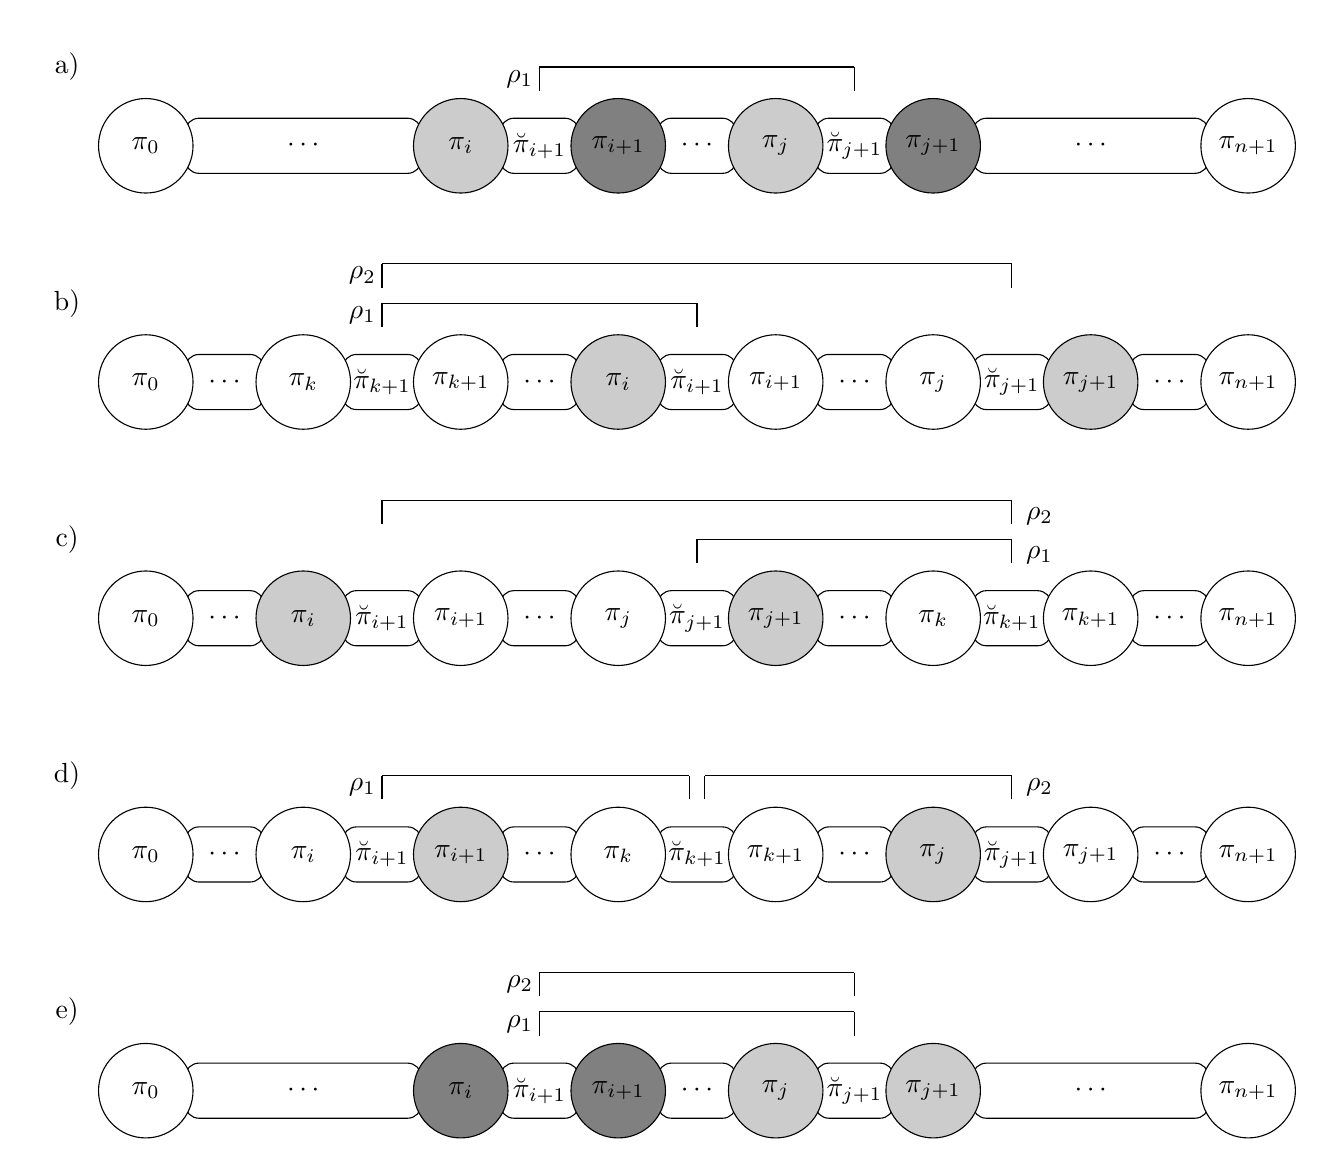
\begin{tikzpicture}
      %%%%% a)

      \node[draw=none,fill=none, minimum height=1cm, minimum width=1cm] at (-3.0, 1.0) {a)};

      % intergenic regions
      \node[rectangle,draw,fill=white!20, minimum height=.7cm, minimum width=3cm, rounded corners=5pt] at (0.0, 0.0) {$\cdots$};
      \node[rectangle,draw,fill=white!20, minimum height=.7cm, minimum width=1cm, rounded corners=5pt] at (3.0, 0.0) {$\breve\pi_{i+1}$};
      \node[rectangle,draw,fill=white!20, minimum height=.7cm, minimum width=1cm, rounded corners=5pt] at (5.0, 0.0) {$\cdots$};
      \node[rectangle,draw,fill=white!20, minimum height=.7cm, minimum width=1cm, rounded corners=5pt] at (7.0, 0.0) {$\breve\pi_{j+1}$};
      \node[rectangle,draw,fill=white!20, minimum height=.7cm, minimum width=3cm, rounded corners=5pt] at (10.0, 0.0) {$\cdots$};

      % genes
      \node[draw, circle, minimum height=1.2cm, minimum width=1.2cm, fill=white!20] at ({(2*0 - 2)}, 0.0) {$\pi_{0}$};
      \node[draw, circle, minimum height=1.2cm, minimum width=1.2cm, fill=black!20] at ({(2*2 - 2)}, 0.0) {$\pi_{i}$};
      \node[draw, circle, minimum height=1.2cm, minimum width=1.2cm, fill=black!50] at ({(2*3 - 2)}, 0.0) {$\pi_{i+1}$};
      \node[draw, circle, minimum height=1.2cm, minimum width=1.2cm, fill=black!20] at ({(2*4 - 2)}, 0.0) {$\pi_{j}$};
      \node[draw, circle, minimum height=1.2cm, minimum width=1.2cm, fill=black!50] at ({(2*5 - 2)}, 0.0) {$\pi_{j+1}$};
      \node[draw, circle, minimum height=1.2cm, minimum width=1.2cm, fill=white!20] at ({(2*7 - 2)}, 0.0) {$\pi_{n+1}$};

      % indexes
      \draw (3.0, 0.7) -- (3.0, 1.0);
      \draw (7.0, 0.7) -- (7.0, 1.0);
      \draw (3.0, 1.0) -- (7.0, 1.0);
      \node[draw=none,fill=none] at (2.75, 0.85) {$\rho_1$};

      %%%%% b)

      \node[draw=none,fill=none, minimum height=1cm, minimum width=1cm] at (-3.0, -2.0) {b)};

      % intergenic regions
      \node[rectangle,draw,fill=white!20, minimum height=.7cm, minimum width=1cm, rounded corners=5pt] at (-1.0, -3.0) {$\cdots$};
      \node[rectangle,draw,fill=white!20, minimum height=.7cm, minimum width=1cm, rounded corners=5pt] at (1.0, -3.0) {$\breve\pi_{k+1}$};
      \node[rectangle,draw,fill=white!20, minimum height=.7cm, minimum width=1cm, rounded corners=5pt] at (3.0, -3.0) {$\cdots$};
      \node[rectangle,draw,fill=white!20, minimum height=.7cm, minimum width=1cm, rounded corners=5pt] at (5.0, -3.0) {$\breve\pi_{i+1}$};
      \node[rectangle,draw,fill=white!20, minimum height=.7cm, minimum width=1cm, rounded corners=5pt] at (7.0, -3.0) {$\cdots$};
      \node[rectangle,draw,fill=white!20, minimum height=.7cm, minimum width=1cm, rounded corners=5pt] at (9.0, -3.0) {$\breve\pi_{j+1}$};
      \node[rectangle,draw,fill=white!20, minimum height=.7cm, minimum width=1cm, rounded corners=5pt] at (11.0, -3.0) {$\cdots$};

      % genes
      \node[draw, circle, minimum height=1.2cm, minimum width=1.2cm, fill=white!20] at ({(2*0 - 2)}, -3.0) {$\pi_{0}$};
      \node[draw, circle, minimum height=1.2cm, minimum width=1.2cm, fill=white!20] at ({(2*1 - 2)}, -3.0) {$\pi_{k}$};
      \node[draw, circle, minimum height=1.2cm, minimum width=1.2cm, fill=white!20] at ({(2*2 - 2)}, -3.0) {$\pi_{k+1}$};
      \node[draw, circle, minimum height=1.2cm, minimum width=1.2cm, fill=black!20] at ({(2*3 - 2)}, -3.0) {$\pi_{i}$};
      \node[draw, circle, minimum height=1.2cm, minimum width=1.2cm, fill=white!20] at ({(2*4 - 2)}, -3.0) {$\pi_{i+1}$};
      \node[draw, circle, minimum height=1.2cm, minimum width=1.2cm, fill=white!20] at ({(2*5 - 2)}, -3.0) {$\pi_{j}$};
      \node[draw, circle, minimum height=1.2cm, minimum width=1.2cm, fill=black!20] at ({(2*6 - 2)}, -3.0) {$\pi_{j+1}$};
      \node[draw, circle, minimum height=1.2cm, minimum width=1.2cm, fill=white!20] at ({(2*7 - 2)}, -3.0) {$\pi_{n+1}$};

      % indexes
      \draw (1.0, -2.3) -- (1.0, -2.0);
      \draw (5.0, -2.3) -- (5.0, -2.0);
      \draw (1.0, -2.0) -- (5.0, -2.0);
      \node[draw=none,fill=none] at (0.75, -2.15) {$\rho_1$};

      \draw (9.0, -1.8) -- (9.0, -1.5);
      \draw (1.0, -1.8) -- (1.0, -1.5);
      \draw (1.0, -1.5) -- (9.0, -1.5);
      \node[draw=none,fill=none] at (0.75, -1.65) {$\rho_2$};

      %%%%% c)

      \node[draw=none,fill=none, minimum height=1cm, minimum width=1cm] at (-3.0, -5.0) {c)};

      % intergenic regions
      \node[rectangle,draw,fill=white!20, minimum height=.7cm, minimum width=1cm, rounded corners=5pt] at (-1.0, -6.0) {$\cdots$};
      \node[rectangle,draw,fill=white!20, minimum height=.7cm, minimum width=1cm, rounded corners=5pt] at (1.0, -6.0) {$\breve\pi_{i+1}$};
      \node[rectangle,draw,fill=white!20, minimum height=.7cm, minimum width=1cm, rounded corners=5pt] at (3.0, -6.0) {$\cdots$};
      \node[rectangle,draw,fill=white!20, minimum height=.7cm, minimum width=1cm, rounded corners=5pt] at (5.0, -6.0) {$\breve\pi_{j+1}$};
      \node[rectangle,draw,fill=white!20, minimum height=.7cm, minimum width=1cm, rounded corners=5pt] at (7.0, -6.0) {$\cdots$};
      \node[rectangle,draw,fill=white!20, minimum height=.7cm, minimum width=1cm, rounded corners=5pt] at (9.0, -6.0) {$\breve\pi_{k+1}$};
      \node[rectangle,draw,fill=white!20, minimum height=.7cm, minimum width=1cm, rounded corners=5pt] at (11.0, -6.0) {$\cdots$};

      % genes
      \node[draw, circle, minimum height=1.2cm, minimum width=1.2cm, fill=white!20] at ({(2*0 - 2)}, -6.0) {$\pi_{0}$};
      \node[draw, circle, minimum height=1.2cm, minimum width=1.2cm, fill=black!20] at ({(2*1 - 2)}, -6.0) {$\pi_{i}$};
      \node[draw, circle, minimum height=1.2cm, minimum width=1.2cm, fill=white!20] at ({(2*2 - 2)}, -6.0) {$\pi_{i+1}$};
      \node[draw, circle, minimum height=1.2cm, minimum width=1.2cm, fill=white!20] at ({(2*3 - 2)}, -6.0) {$\pi_{j}$};
      \node[draw, circle, minimum height=1.2cm, minimum width=1.2cm, fill=black!20] at ({(2*4 - 2)}, -6.0) {$\pi_{j+1}$};
      \node[draw, circle, minimum height=1.2cm, minimum width=1.2cm, fill=white!20] at ({(2*5 - 2)}, -6.0) {$\pi_{k}$};
      \node[draw, circle, minimum height=1.2cm, minimum width=1.2cm, fill=white!20] at ({(2*6 - 2)}, -6.0) {$\pi_{k+1}$};
      \node[draw, circle, minimum height=1.2cm, minimum width=1.2cm, fill=white!20] at ({(2*7 - 2)}, -6.0) {$\pi_{n+1}$};

      % indexes
      \draw (5.0, -5.3) -- (5.0, -5.0);
      \draw (9.0, -5.3) -- (9.0, -5.0);
      \draw (5.0, -5.0) -- (9.0, -5.0);
      \node[draw=none,fill=none] at (9.35, -5.2) {$\rho_1$};

      \draw (9.0, -4.8) -- (9.0, -4.5);
      \draw (1.0, -4.8) -- (1.0, -4.5);
      \draw (1.0, -4.5) -- (9.0, -4.5);
      \node[draw=none,fill=none] at (9.35, -4.7) {$\rho_2$};

      %%%%% d)

      \node[draw=none,fill=none, minimum height=1cm, minimum width=1cm] at (-3.0, -8.0) {d)};

      % intergenic regions
      \node[rectangle,draw,fill=white!20, minimum height=.7cm, minimum width=1cm, rounded corners=5pt] at (-1.0, -9.0) {$\cdots$};
      \node[rectangle,draw,fill=white!20, minimum height=.7cm, minimum width=1cm, rounded corners=5pt] at (1.0, -9.0) {$\breve\pi_{i+1}$};
      \node[rectangle,draw,fill=white!20, minimum height=.7cm, minimum width=1cm, rounded corners=5pt] at (3.0, -9.0) {$\cdots$};
      \node[rectangle,draw,fill=white!20, minimum height=.7cm, minimum width=1cm, rounded corners=5pt] at (5.0, -9.0) {$\breve\pi_{k+1}$};
      \node[rectangle,draw,fill=white!20, minimum height=.7cm, minimum width=1cm, rounded corners=5pt] at (7.0, -9.0) {$\cdots$};
      \node[rectangle,draw,fill=white!20, minimum height=.7cm, minimum width=1cm, rounded corners=5pt] at (9.0, -9.0) {$\breve\pi_{j+1}$};
      \node[rectangle,draw,fill=white!20, minimum height=.7cm, minimum width=1cm, rounded corners=5pt] at (11.0, -9.0) {$\cdots$};

      % genes
      \node[draw, circle, minimum height=1.2cm, minimum width=1.2cm, fill=white!20] at ({(2*0 - 2)}, -9.0) {$\pi_{0}$};
      \node[draw, circle, minimum height=1.2cm, minimum width=1.2cm, fill=white!20] at ({(2*1 - 2)}, -9.0) {$\pi_{i}$};
      \node[draw, circle, minimum height=1.2cm, minimum width=1.2cm, fill=black!20] at ({(2*2 - 2)}, -9.0) {$\pi_{i+1}$};
      \node[draw, circle, minimum height=1.2cm, minimum width=1.2cm, fill=white!20] at ({(2*3 - 2)}, -9.0) {$\pi_{k}$};
      \node[draw, circle, minimum height=1.2cm, minimum width=1.2cm, fill=white!20] at ({(2*4 - 2)}, -9.0) {$\pi_{k+1}$};
      \node[draw, circle, minimum height=1.2cm, minimum width=1.2cm, fill=black!20] at ({(2*5 - 2)}, -9.0) {$\pi_{j}$};
      \node[draw, circle, minimum height=1.2cm, minimum width=1.2cm, fill=white!20] at ({(2*6 - 2)}, -9.0) {$\pi_{j+1}$};
      \node[draw, circle, minimum height=1.2cm, minimum width=1.2cm, fill=white!20] at ({(2*7 - 2)}, -9.0) {$\pi_{n+1}$};

      % indexes
      \draw (1.0, -8.3) -- (1.0, -8.0);
      \draw (4.9, -8.3) -- (4.9, -8.0);
      \draw (1.0, -8.0) -- (4.9, -8.0);
      \node[draw=none,fill=none] at (0.75, -8.15) {$\rho_1$};

      \draw (5.1, -8.3) -- (5.1, -8.0);
      \draw (9.0, -8.3) -- (9.0, -8.0);
      \draw (5.1, -8.0) -- (9.0, -8.0);
      \node[draw=none,fill=none] at (9.35, -8.15) {$\rho_2$};

      %%%%% e)

      \node[draw=none,fill=none, minimum height=1cm, minimum width=1cm] at (-3.0, -11.0) {e)};

      % intergenic regions
      \node[rectangle,draw,fill=white!20, minimum height=.7cm, minimum width=3cm, rounded corners=5pt] at (0.0, -12.0) {$\cdots$};
      \node[rectangle,draw,fill=white!20, minimum height=.7cm, minimum width=1cm, rounded corners=5pt] at (3.0, -12.0) {$\breve\pi_{i+1}$};
      \node[rectangle,draw,fill=white!20, minimum height=.7cm, minimum width=1cm, rounded corners=5pt] at (5.0, -12.0) {$\cdots$};
      \node[rectangle,draw,fill=white!20, minimum height=.7cm, minimum width=1cm, rounded corners=5pt] at (7.0, -12.0) {$\breve\pi_{j+1}$};
      \node[rectangle,draw,fill=white!20, minimum height=.7cm, minimum width=3cm, rounded corners=5pt] at (10.0, -12.0) {$\cdots$};

      % genes
      \node[draw, circle, minimum height=1.2cm, minimum width=1.2cm, fill=white!20] at ({(2*0 - 2)}, -12.0) {$\pi_{0}$};
      \node[draw, circle, minimum height=1.2cm, minimum width=1.2cm, fill=black!50] at ({(2*2 - 2)}, -12.0) {$\pi_{i}$};
      \node[draw, circle, minimum height=1.2cm, minimum width=1.2cm, fill=black!50] at ({(2*3 - 2)}, -12.0) {$\pi_{i+1}$};
      \node[draw, circle, minimum height=1.2cm, minimum width=1.2cm, fill=black!20] at ({(2*4 - 2)}, -12.0) {$\pi_{j}$};
      \node[draw, circle, minimum height=1.2cm, minimum width=1.2cm, fill=black!20] at ({(2*5 - 2)}, -12.0) {$\pi_{j+1}$};
      \node[draw, circle, minimum height=1.2cm, minimum width=1.2cm, fill=white!20] at ({(2*7 - 2)}, -12.0) {$\pi_{n+1}$};

      % indexes
      \draw (3.0, -11.3) -- (3.0, -11.0);
      \draw (7.0, -11.3) -- (7.0, -11.0);
      \draw (3.0, -11.0) -- (7.0, -11.0);
      \node[draw=none,fill=none] at (2.75, -11.15) {$\rho_1$};

      \draw (3.0, -10.8) -- (3.0, -10.5);
      \draw (7.0, -10.8) -- (7.0, -10.5);
      \draw (3.0, -10.5) -- (7.0, -10.5);
      \node[draw=none,fill=none] at (2.75, -10.65) {$\rho_2$};
    \end{tikzpicture}
  }
  \caption[Possibilidades de remoção de, pelo menos, um breakpoint tipo um a partir de pares de breakpoints conectados.]{Possibilidades que podem surgir quando existe um par de breakpoints conectados e reversões que podem ser aplicadas para remover, pelo menos, um breakpoint tipo um. O par de elementos consecutivos no genoma alvo está representado por tons de cinza.}
  \label{figure:EMTPDAVS}
\end{figure}

A seguir apresentamos o Algoritmo~\ref{algorithm:AKKUXQNR} para a variação sem sinais do problema \SbIR{}.  

\begin{algorithm}[!tbh]
  \caption{Um algoritmo de aproximação para o problema \SbIR{}.\label{algorithm:AKKUXQNR}}
  \Entrada{Uma instância intergênica rígida balanceada sem sinais $\mathcal{I}=((\pi,\breve\pi),(\iota,\breve\iota))$}
  \Saida{Uma sequência de reversões $S$, tal que $(\pi,\breve\pi) \cdot S = (\iota,\breve\iota)$}
    Seja $S \gets ()$ \\
    \Enqto{$ib_1(\mathcal{I}) > 1$}{
      \tcp{Lema~\ref{lemma:WYEZMYTM}}
      $(\pi_i,\pi_{i+1})$, $(\pi_j,\pi_{j+1}) \gets $ encontre um par de breakpoints conectados \\
      \tcp{Lema~\ref{lemma:IMYFBWDY}}
      \Se{$(\pi_i,\pi_{i+1})$, $(\pi_j,\pi_{j+1})$ pertence ao caso $(i)$}{
        $S' \gets (\rho_1)$ \\
      }\SenaoSe{$(\pi_i,\pi_{i+1})$, $(\pi_j,\pi_{j+1})$ pertence ao caso $(ii)$}{
        $S' \gets (\rho_1,\rho_2)$ \\
      }\SenaoSe{$(\pi_i,\pi_{i+1})$, $(\pi_j,\pi_{j+1})$ pertence ao caso $(iii)$}{
        $S' \gets (\rho_1,\rho_2)$ \\
      }\SenaoSe{$(\pi_i,\pi_{i+1})$, $(\pi_j,\pi_{j+1})$ pertence ao caso $(iv)$}{
        $S' \gets (\rho_1,\rho_2)$ \\
      }
      $S \gets S + S'$ \\
      $\mathcal{I} \gets ((\pi, \breve\pi) \cdot S',(\iota,\breve\iota))$ \\
    }
  \Retorna{S}
\end{algorithm}

\begin{lemma}\label{lemma:RBHACFIP}
Dada uma instância intergênica rígida balanceada sem sinais $\mathcal{I}=((\pi,\breve\pi),\break(\iota,\breve\iota))$, o Algoritmo~\ref{algorithm:AKKUXQNR} transforma $(\pi,\breve\pi)$ em $(\iota,\breve\iota)$ utilizando no máximo $2ib_1(\mathcal{I})$ reversões.
\end{lemma}
\begin{proof}
  No Algoritmo~\ref{algorithm:AKKUXQNR}, temos que enquanto $ib_1(\mathcal{I})$ for maior que um, ou seja, $(\pi,\breve\pi)$ for diferente de $(\iota,\breve\iota)$ (pela Observação~\ref{remark:UDYJTHAH} e Lema~\ref{lemma:WSPRPLAH}), o seguinte procedimento é aplicado: pelos lemas~\ref{lemma:WYEZMYTM} e~\ref{lemma:IMYFBWDY}, sempre podemos encontrar um par conectado de breakpoints e remover pelo menos um breakpoint tipo um após aplicar no máximo duas reversões. A cada iteração do algoritmo pelo menos um breakpoint tipo um é removido. Dessa forma, o genoma alvo eventualmente será alcançado. No pior caso, cada breakpoint tipo um é removido utilizando duas reversões. Logo, $2ib_1(\mathcal{I})$ reversões, no máximo, são utilizadas para transformar $(\pi,\breve\pi)$ em $(\iota,\breve\iota)$ e o lema segue.
\end{proof}

Note que o Algoritmo~\ref{algorithm:AKKUXQNR} pode ser analisado considerando os seguintes pontos: 
\begin{itemize}
  \item Encontrar o par conectado de breakpoints, que pode ser feito em tempo linear com o auxílio da permutação inversa de $\pi$.
  \item Aplicação dos casos do Lema~\ref{lemma:IMYFBWDY}, que no pior caso, também pode levar um tempo linear se for necessário encontrar o breakpoint tipo um $(\pi_k,\pi_{k+1})$ nos casos $ii$ e $iii$. 
\end{itemize}
Como esse processo é repetido no máximo $n$ vezes, então o tempo de execução do Algoritmo~\ref{algorithm:AKKUXQNR} é $\mathcal{O}(n^2)$.

\begin{theorem}\label{theorem:BLJAGNDZ}
Dada uma instância intergênica rígida balanceada sem sinais $\mathcal{I}=\break((\pi,\breve\pi),(\iota,\breve\iota))$, o Algoritmo~\ref{algorithm:AKKUXQNR} é uma $4$-aproximação para o problema \SbIR{}.
\end{theorem}
\begin{proof}
Pelo Lema~\ref{lemma:RBHACFIP}, o Algoritmo~\ref{algorithm:AKKUXQNR} transforma $(\pi,\breve\pi)$ em $(\iota,\breve\iota)$ utilizando no máximo $2ib_1(\mathcal{I})$ reversões. Pelo Teorema~\ref{theorem:MPFPKHQO}, temos o seguinte limitante inferior $d_{\SbIR}(\mathcal{I}) \ge \frac{ib_1(\mathcal{I})}{2}$. Logo, o teorema segue. 
\end{proof}

% ------------------------------------------------------------------ %
\subsection{Reversão e Indel}
% ------------------------------------------------------------------ %

Nesta seção apresentaremos um algoritmo de aproximação com fator $4$ para a variação sem sinais do problema \SbIRI{}.

\begin{lemma}\label{lemma:QGOIQLZD}
Dada uma instância intergênica rígida desbalanceada sem sinais $\mathcal{I}=((\pi,\breve\pi),\break(\iota,\breve\iota))$, tal que $\sum_{i=1}^{n+1}\breve\pi_i < \sum_{i=1}^{n+1}\breve\iota_i$, então sempre é possível aplicar um indel $\delta$ de forma que $\Delta ib_1(\mathcal{I}, S=(\delta)) \le 0$ e $\mathcal{I}$ é tranformada em uma instância intergênica rígida balanceada.
\end{lemma}
\begin{proof}
Como $\mathcal{I}$ é desbalanceada, então $ib_1(\mathcal{I}) > 0$. Seja $(\pi_i,\pi_{i+1})$ um breakpoint tipo um de $\mathcal{I}$. Aplique o indel $\delta_{(x)}^{(i+1)}$, tal que $x = \sum_{i=1}^{n+1}\breve\iota_i - \sum_{i=1}^{n+1}\breve\pi_i$. Note que o indel insere a quantidade necessária de nucleotídeos na região intergênica $\breve\pi_{i+1}$ para tornar $\mathcal{I}$ uma instância balanceada. No pior caso, $(\pi_i,\pi_{i+1})$ continua sendo um breakpoint tipo um e o lema segue.
\end{proof}

\begin{lemma}\label{lemma:QNHGBLYF}
Dada uma instância intergênica rígida desbalanceada sem sinais $\mathcal{I}=((\pi,\breve\pi),\break(\iota,\breve\iota))$, tal que $ib_1(\mathcal{I}) = 1$, então sempre é possível aplicar um indel $\delta$ de forma que $\Delta ib_1(\mathcal{I}, S=(\delta)) = -1$.
\end{lemma}
\begin{proof}
Seja $(\pi_i,\pi_{i+1})$ o único breakpoint tipo um de $\mathcal{I}$. Como $(\pi_i,\pi_{i+1})$ é único breakpoint tipo um de $\mathcal{I}$, então obrigatoriamente ele deve ser um breakpoint forte. Aplique o indel $\delta_{(x)}^{(i+1)}$, tal que $x = \breve\iota_{i+1} - \breve\pi_{i+1}$. Note que o indel insere ou remove a quantidade necessária de nucleotídeos na região intergênica $\breve\pi_{i+1}$ para remover o breakpoint $(\pi_i,\pi_{i+1})$ caso ele seja subcarregado ou sobrecarregado, respectivamente. Como o breakpoint $(\pi_i,\pi_{i+1})$ acaba sendo removido após a aplicação do evento de indel, o lema segue.
\end{proof}

A seguir apresentamos o Algoritmo~\ref{algorithm:LHOPSFVN} para a variação sem sinais do problema \SbIRI{}.

\begin{algorithm}[!tbh]
  \caption{Um algoritmo de aproximação para o problema \SbIRI{}.\label{algorithm:LHOPSFVN}}
  \Entrada{Uma instância intergênica rígida sem sinais $\mathcal{I}=((\pi,\breve\pi),(\iota,\breve\iota))$}
  \Saida{Uma sequência de reversões e indels $S$, tal que $(\pi,\breve\pi) \cdot S = (\iota,\breve\iota)$}
    Seja $S \gets ()$ \\
    \tcp{Lema~\ref{lemma:QGOIQLZD}}
    \Se{$\sum_{i=1}^{n+1}\breve\pi_i < \sum_{i=1}^{n+1}\breve\iota_i$}{
      $S' \gets (\delta_1)$ \\
      $S \gets S + S'$ \\
      $\mathcal{I} \gets ((\pi, \breve\pi) \cdot S',(\iota,\breve\iota))$ \\
    }
    \Enqto{$ib(\mathcal{I}) > 1$}{
      \tcp{Lema~\ref{lemma:WYEZMYTM}}
      $(\pi_i,\pi_{i+1})$, $(\pi_j,\pi_{j+1}) \gets $ encontre um par de breakpoints conectados \\
      \tcp{Lema~\ref{lemma:IMYFBWDY}}
      \Se{$(\pi_i,\pi_{i+1})$, $(\pi_j,\pi_{j+1})$ pertence ao caso $(i)$}{
        $S' \gets (\rho_1)$ \\
      }\SenaoSe{$(\pi_i,\pi_{i+1})$, $(\pi_j,\pi_{j+1})$ pertence ao caso $(ii)$}{
        $S' \gets (\rho_1,\rho_2)$ \\
      }\SenaoSe{$(\pi_i,\pi_{i+1})$, $(\pi_j,\pi_{j+1})$ pertence ao caso $(iii)$}{
        $S' \gets (\rho_1,\rho_2)$ \\
      }\SenaoSe{$(\pi_i,\pi_{i+1})$, $(\pi_j,\pi_{j+1})$ pertence ao caso $(iv)$}{
        $S' \gets (\rho_1,\rho_2)$ \\
      }
      $S \gets S + S'$ \\
      $\mathcal{I} \gets ((\pi, \breve\pi) \cdot S',(\iota,\breve\iota))$ \\
    }
    \tcp{Lema~\ref{lemma:QNHGBLYF}}
    \Se{$ib(\mathcal{I}) = 1$}{
      $S' \gets (\delta_1)$ \\
      $S \gets S + S'$ \\
      $\mathcal{I} \gets ((\pi, \breve\pi) \cdot S',(\iota,\breve\iota))$ \\
    }
  \Retorna{S}
\end{algorithm}

\begin{lemma}\label{lemma:XUDIVWPC}
Dada uma instância intergênica rígida sem sinais $\mathcal{I}=((\pi,\breve\pi),(\iota,\breve\iota))$, o Algoritmo~\ref{algorithm:LHOPSFVN} transforma $(\pi,\breve\pi)$ em $(\iota,\breve\iota)$ utilizando no máximo $2ib_1(\mathcal{I})$ eventos de reversão e indel.
\end{lemma}
\begin{proof}
  Podemos analisar o Algoritmo~\ref{algorithm:LHOPSFVN} considerando três cenários:
  \begin{itemize}
    \item $\sum_{i=1}^{n+1}\breve\pi_i < \sum_{i=1}^{n+1}\breve\iota_i$, neste cenários o Algoritmo~\ref{algorithm:LHOPSFVN} aplica um indel (linhas 2-5) que pode não remover nenhum breakpoint tipo um, mas torna $\mathcal{I}$ em uma instância balanceada. Caso ainda existam breakpoints em $\mathcal{I}$, então o laço de repetição (linhas 6-17) remove, por iteração, pelo menos um breakpoint tipo um utilizando no máximo duas reversões. Esse processo repete-se até que todos os breakpoints tipo um de $\mathcal{I}$ sejam removidos. Como todos os breakpoints tipo um são removidos, então $(\pi,\breve\pi)$ é transformada em $(\iota,\breve\iota)$. Note que se o indel aplicado inicialmente não remover nenhum breakpoint tipo um, então pelo menos uma reversão é aplicada em seguida. Além disso, pelo Lema~\ref{lemma:WSPRPLAH}, podemos deduzir que a última reversão que transforma $(\pi,\breve\pi)$ em $(\iota,\breve\iota)$ deve obrigatoriamente remover dois breakpoints tipo um. Isso implica que no máximo $2ib_1(\mathcal{I})$ reversões e indels são utilizadas pelo Algoritmo~\ref{algorithm:LHOPSFVN} para transformar $(\pi,\breve\pi)$ em $(\iota,\breve\iota)$.
    \item $\sum_{i=1}^{n+1}\breve\pi_i = \sum_{i=1}^{n+1}\breve\iota_i$, para esse cenários o Algoritmo~\ref{algorithm:LHOPSFVN} comporta-se exatamente como o Algoritmo~\ref{algorithm:AKKUXQNR}, que transforma $(\pi,\breve\pi)$ em $(\iota,\breve\iota)$ utilizando no máximo $2ib_1(\mathcal{I})$ reversões.
    \item $\sum_{i=1}^{n+1}\breve\pi_i > \sum_{i=1}^{n+1}\breve\iota_i$, neste último cenário enquanto $ib(\mathcal{I})$ for maior que um, o Algoritmo~\ref{algorithm:LHOPSFVN} aplica no máximo duas reversões a cada iteração do laço de repetição (linhas 6-17) que removem pelo menos um breakpoint tipo um. Por fim, um indel é aplicado (linhas 19-22) transformando $(\pi,\breve\pi)$ em $(\iota,\breve\iota)$. Note que no pior caso deste cenário cada breakpoint tipo um é removido após a aplicação de duas reversões.
  \end{itemize}
  Nos três cenários o Algoritmo~\ref{algorithm:LHOPSFVN} transforma $(\pi,\breve\pi)$ em $(\iota,\breve\iota)$ utilizando no máximo $2ib_1(\mathcal{I})$ reversões e indels e o lema segue.
\end{proof}

Note que o Algoritmo~\ref{algorithm:LHOPSFVN} difere do Algoritmo~\ref{algorithm:AKKUXQNR} pelos trechos responsáveis por aplicar uma operção de indel (linhas 2-5 e 19-22). Ambos os trechos podem ser realizar em tempo linear. Dessa forma, o tempo de execução do Algoritmo~\ref{algorithm:LHOPSFVN} também é $\mathcal{O}(n^2)$.

\begin{theorem}\label{theorem:AFAHUIUF}
Dada uma instância intergênica rígida sem sinais $\mathcal{I}=((\pi,\breve\pi),(\iota,\breve\iota))$, o Algoritmo~\ref{algorithm:LHOPSFVN} é uma $4$-aproximação para o problema \SbIRI{}.
\end{theorem}
\begin{proof}
Pelo Lema~\ref{lemma:XUDIVWPC}, o Algoritmo~\ref{algorithm:LHOPSFVN} transforma $(\pi,\breve\pi)$ em $(\iota,\breve\iota)$ utilizando no máximo $2ib_1(\mathcal{I})$ eventos de reversão e indel. Pelo Teorema~\ref{theorem:MPFPKHQO}, temos o seguinte limitante inferior $d_{\SbIRI}(\mathcal{I}) \ge \frac{ib_1(\mathcal{I})}{2}$. Logo, o teorema segue. 
\end{proof}

% ------------------------------------------------------------------ %
\subsection{Reversão e Move}
% ------------------------------------------------------------------ %

Nesta seção apresentaremos um algoritmo de aproximação com fator $4$ para a variação sem sinais do problema \SbIRM{}.

\begin{lemma}\label{lemma:NWNNZGXH}
Dada uma instância intergênica rígida sem sinais $\mathcal{I}=((\pi,\breve\pi),(\iota,\breve\iota))$ e sejam $(\pi_i,\pi_{i+1})$ e $(\pi_j,\pi_{j+1})$ breakpoints conectados, então é possível remover pelo menos um breakpoint tipo um de $\mathcal{I}$ utilizando no máximo duas reversões ou um move.
\end{lemma}
\begin{proof}
Note a aplicação do Lema~\ref{lemma:IMYFBWDY} já é suficiente para provar este lema. Entretanto, iremos melhorar o caso $iv$ para utilizarmos apenas um evento de move ao invés de duas reversões. Sem perda de generalidade assuma que $i < j$, como o par de breakpoints $(\pi_i,\pi_{i+1})$ e $(\pi_j,\pi_{j+1})$ está conectado, por definição, uma das seguintes possibilidades deve ocorrer:
\begin{enumerate}[i.]
  \item O par de elementos $(\pi_i,\pi_{j})$ ou $(\pi_{i+1},\pi_{j+1})$ não formam uma adjacência intergênica, são consecutivos em $\iota$ e $\breve\pi_{i+1} + \breve\pi_{j+1} \ge \breve\iota_k$, onde $\breve\iota_k$ é o tamanho da região intergênica entre o par de elementos consecutivos em $\iota$. Aplique uma reversão como descrito no caso $i$ do Lema~\ref{lemma:IMYFBWDY}.   
  \item O par  de elementos $(\pi_i,\pi_{j+1})$ não formam uma adjacência intergênica, são consecutivos em $\iota$ e $\breve\pi_{i+1} + \breve\pi_{j+1} \ge \breve\iota_k$, onde $\breve\iota_k$ é o tamanho da região intergênica entre o par de elementos consecutivos em $\iota$. Aplique uma sequência de duas reversões como descrito no caso $ii$ do Lema~\ref{lemma:IMYFBWDY}.
  \item O par de elementos $(\pi_{i+1},\pi_{j})$ não formam uma adjacência intergênica, são consecutivos em $\iota$ e $\breve\pi_{i+1} + \breve\pi_{j+1} \ge \breve\iota_k$, onde $\breve\iota_k$ é o tamanho da região intergênica entre o par de elementos consecutivos em $\iota$. Aplique uma sequência de duas reversões como descrito no caso $iii$ do Lema~\ref{lemma:IMYFBWDY}.
  \item O par de elementos $(\pi_{i},\pi_{i+1})$ ou $(\pi_{j},\pi_{j+1})$ não formam uma adjacência intergênica, são consecutivos em $\iota$ e $\breve\pi_{i+1} + \breve\pi_{j+1} \ge \breve\iota_k$, onde $\breve\iota_k$ é o tamanho da região intergênica entre o par de elementos consecutivos em $\iota$. Neste caso, obrigatoriamente $(\pi_{i},\pi_{i+1})$ ou $(\pi_{j},\pi_{j+1})$ deve ser um breakpoint forte. Se $(\pi_{i},\pi_{i+1})$ for um breakpoint forte, então ele pode ser sobrecarregado ou subcarregado. Caso ele seja sobrecarregado, então aplicamos um move $\mu^{(i+1,j+1)_{(x)}}$, tal que $x = \breve\pi_{i+1} - \breve\iota_{max(\pi_{i},\pi_{i+1})}$. Caso contrário, aplicamos um move $\mu^{(j+1,i+1)_{(x)}}$, tal que $x = \breve\iota_{max(\pi_{i},\pi_{i+1})} - \breve\pi_{i+1}$. De maneira similar, se $(\pi_{j},\pi_{j+1})$ for um breakpoint forte, então ele pode ser sobrecarregado ou subcarregado. Caso ele seja sobrecarregado, então aplicamos um move $\mu^{(j+1,i+1)_{(x)}}$, tal que $x = \breve\pi_{j+1} - \breve\iota_{max(\pi_{j},\pi_{j+1})}$. Caso contrário, aplicamos um move $\mu^{(i+1,j+1)_{(x)}}$, tal que $x = \breve\iota_{max(\pi_{j},\pi_{j+1})} - \breve\pi_{j+1}$. Em ambos os cenários pelo menos um breakpoint tipo um é removido após a aplicação do move (Figura~\ref{figure:CAIZFSWA}).
\end{enumerate}
Note que o caso $(i)$ aplica apenas um reversão e remove pelo menos um breakpoint tipo um. Os casos $(ii)$ e $(iii)$ aplicam inicialmente uma reversão que não remove nenhum breakpoint tipo um, mas garatem que nenhum novo breakpoint é gerado e o caso $(i)$ poderá ser aplicado em seguida. Por fim, o caso $(iv)$ remove pelo menos um breakpoint tipo um utilizando um move. No pior caso duas reversões são aplicadas e pelo menos um breakpoint tipo um é removido de $\mathcal{I}$. Logo, o lema segue. 
\end{proof}

\begin{figure}[!tbh]
  \resizebox{\linewidth}{!}{
    \centering
    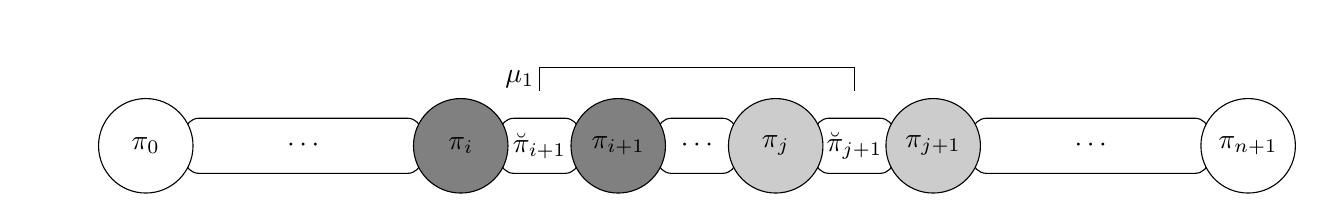
\begin{tikzpicture}
      %%%%% e)

      \node[draw=none,fill=none, minimum height=1cm, minimum width=1cm] at (-3.0, -11.0) {};

      % intergenic regions
      \node[rectangle,draw,fill=white!20, minimum height=.7cm, minimum width=3cm, rounded corners=5pt] at (0.0, -12.0) {$\cdots$};
      \node[rectangle,draw,fill=white!20, minimum height=.7cm, minimum width=1cm, rounded corners=5pt] at (3.0, -12.0) {$\breve\pi_{i+1}$};
      \node[rectangle,draw,fill=white!20, minimum height=.7cm, minimum width=1cm, rounded corners=5pt] at (5.0, -12.0) {$\cdots$};
      \node[rectangle,draw,fill=white!20, minimum height=.7cm, minimum width=1cm, rounded corners=5pt] at (7.0, -12.0) {$\breve\pi_{j+1}$};
      \node[rectangle,draw,fill=white!20, minimum height=.7cm, minimum width=3cm, rounded corners=5pt] at (10.0, -12.0) {$\cdots$};

      % genes
      \node[draw, circle, minimum height=1.2cm, minimum width=1.2cm, fill=white!20] at ({(2*0 - 2)}, -12.0) {$\pi_{0}$};
      \node[draw, circle, minimum height=1.2cm, minimum width=1.2cm, fill=black!50] at ({(2*2 - 2)}, -12.0) {$\pi_{i}$};
      \node[draw, circle, minimum height=1.2cm, minimum width=1.2cm, fill=black!50] at ({(2*3 - 2)}, -12.0) {$\pi_{i+1}$};
      \node[draw, circle, minimum height=1.2cm, minimum width=1.2cm, fill=black!20] at ({(2*4 - 2)}, -12.0) {$\pi_{j}$};
      \node[draw, circle, minimum height=1.2cm, minimum width=1.2cm, fill=black!20] at ({(2*5 - 2)}, -12.0) {$\pi_{j+1}$};
      \node[draw, circle, minimum height=1.2cm, minimum width=1.2cm, fill=white!20] at ({(2*7 - 2)}, -12.0) {$\pi_{n+1}$};

      % indexes
      \draw (3.0, -11.3) -- (3.0, -11.0);
      \draw (7.0, -11.3) -- (7.0, -11.0);
      \draw (3.0, -11.0) -- (7.0, -11.0);
      \node[draw=none,fill=none] at (2.75, -11.15) {$\mu_1$};
    \end{tikzpicture}
  }
  \caption[Exemplo de remoção de pelo menos um breakpoint tipo um após a aplicação de um move $\mu$.]{Exemplo de remoção de pelo menos um breakpoint tipo um após a aplicação de um move $\mu$.}
  \label{figure:CAIZFSWA}
\end{figure}

A seguir apresentamos o Algoritmo~\ref{algorithm:OLSRUEFZ} para a variação sem sinais do problema \SbIRM{}.  

\begin{algorithm}[!tbh]
  \caption{Um algoritmo de aproximação para o problema \SbIRM{}.\label{algorithm:OLSRUEFZ}}
  \Entrada{Uma instância intergênica rígida balanceada sem sinais $\mathcal{I}=((\pi,\breve\pi),(\iota,\breve\iota))$}
  \Saida{Uma sequência de reversões e moves $S$, tal que $(\pi,\breve\pi) \cdot S = (\iota,\breve\iota)$}
    Seja $S \gets ()$ \\
    \Enqto{$ib_1(\mathcal{I}) > 1$}{
      \tcp{Lema~\ref{lemma:WYEZMYTM}}
      $(\pi_i,\pi_{i+1})$, $(\pi_j,\pi_{j+1}) \gets $ encontre um par de breakpoints conectados \\
      \tcp{Lema~\ref{lemma:NWNNZGXH}}
      \Se{$(\pi_i,\pi_{i+1})$, $(\pi_j,\pi_{j+1})$ pertence ao caso $(i)$}{
        $S' \gets (\rho_1)$ \\
      }\SenaoSe{$(\pi_i,\pi_{i+1})$, $(\pi_j,\pi_{j+1})$ pertence ao caso $(iv)$}{
        $S' \gets (\mu_1)$ \\
      }
      \SenaoSe{$(\pi_i,\pi_{i+1})$, $(\pi_j,\pi_{j+1})$ pertence ao caso $(ii)$}{
        $S' \gets (\rho_1,\rho_2)$ \\
      }\SenaoSe{$(\pi_i,\pi_{i+1})$, $(\pi_j,\pi_{j+1})$ pertence ao caso $(iii)$}{
        $S' \gets (\rho_1,\rho_2)$ \\
      }
      $S \gets S + S'$ \\
      $\mathcal{I} \gets ((\pi, \breve\pi) \cdot S',(\iota,\breve\iota))$ \\
    }
  \Retorna{S}
\end{algorithm}

\begin{lemma}\label{lemma:TZYVWBRT}
Dada uma instância intergênica rígida balanceada sem sinais $\mathcal{I}=((\pi,\breve\pi),\break(\iota,\breve\iota))$, o Algoritmo~\ref{algorithm:OLSRUEFZ} transforma $(\pi,\breve\pi)$ em $(\iota,\breve\iota)$ utilizando no máximo $2ib_1(\mathcal{I})$ eventos de reversão e move.
\end{lemma}
\begin{proof}
  No Algoritmo~\ref{algorithm:OLSRUEFZ}, temos que enquanto $ib_1(\mathcal{I})$ for maior que um, ou seja, $(\pi,\breve\pi)$ for diferente de $(\iota,\breve\iota)$ (pela Observação~\ref{remark:UDYJTHAH} e Lema~\ref{lemma:WSPRPLAH}), o seguinte procedimento é aplicado: pelos lemas~\ref{lemma:WYEZMYTM} e~\ref{lemma:NWNNZGXH}, sempre podemos encontrar um par conectado de breakpoints e remover pelo menos um breakpoint tipo um após aplicar no máximo duas reversões ou um move. A cada iteração do algoritmo pelo menos um breakpoint tipo um é removido. Dessa forma, o genoma alvo eventualmente será alcançado. No pior caso, cada breakpoint tipo um é removido utilizando dois eventos de rearranjo. Logo, uma sequência com, no máximo, $2ib_1(\mathcal{I})$ reversões e moves é utilizada para transformar $(\pi,\breve\pi)$ em $(\iota,\breve\iota)$ e o lema segue.
\end{proof}

Note que o Algoritmo~\ref{algorithm:OLSRUEFZ} difere do Algoritmo~\ref{algorithm:AKKUXQNR} apenas pelo caso $iv$ de um par conectado de breakpoints, que também pode ser realizado em tempo constante. Logo, o tempo de execução do Algoritmo~\ref{algorithm:OLSRUEFZ} também é $\mathcal{O}(n^2)$.

\begin{theorem}\label{theorem:PNTKLAHZ}
Dada uma instância intergênica rígida balanceada sem sinais $\mathcal{I}=\break((\pi,\breve\pi),(\iota,\breve\iota))$, o Algoritmo~\ref{algorithm:OLSRUEFZ} é uma $4$-aproximação para o problema \SbIRM{}.
\end{theorem}
\begin{proof}
Pelo Lema~\ref{lemma:TZYVWBRT}, o Algoritmo~\ref{algorithm:OLSRUEFZ} transforma $(\pi,\breve\pi)$ em $(\iota,\breve\iota)$ utilizando no máximo $2ib_1(\mathcal{I})$ eventos de reversão e move. Pelo Teorema~\ref{theorem:MPFPKHQO}, temos o seguinte limitante inferior $d_{\SbIRM}(\mathcal{I}) \ge \frac{ib_1(\mathcal{I})}{2}$. Logo, o teorema segue. 
\end{proof}

% ------------------------------------------------------------------ %
\subsection{Reversão, Move e Indel}
% ------------------------------------------------------------------ %

Nesta seção apresentaremos um algoritmo de aproximação com fator $4$ para a variação sem sinais do problema \SbIRMI{}. 

A seguir apresentamos o Algoritmo~\ref{algorithm:JAJGNYWD} para a variação sem sinais do problema \SbIRMI{}.

\begin{algorithm}[!tbh]
  \caption{Um algoritmo de aproximação para o problema \SbIRMI{}.\label{algorithm:JAJGNYWD}}
  \Entrada{Uma instância intergênica rígida sem sinais $\mathcal{I}=((\pi,\breve\pi),(\iota,\breve\iota))$}
  \Saida{Uma sequência de reversões, moves e indels $S$, tal que $(\pi,\breve\pi) \cdot S = (\iota,\breve\iota)$}
    Seja $S \gets ()$ \\
    \tcp{Lema~\ref{lemma:QGOIQLZD}}
    \Se{$\sum_{i=1}^{n+1}\breve\pi_i < \sum_{i=1}^{n+1}\breve\iota_i$}{
      $S' \gets (\delta_1)$ \\
      $S \gets S + S'$ \\
      $\mathcal{I} \gets ((\pi, \breve\pi) \cdot S',(\iota,\breve\iota))$ \\
    }
    \Enqto{$ib(\mathcal{I}) > 1$}{
      \tcp{Lema~\ref{lemma:WYEZMYTM}}
      $(\pi_i,\pi_{i+1})$, $(\pi_j,\pi_{j+1}) \gets $ encontre um par de breakpoints conectados \\
      \tcp{Lema~\ref{lemma:NWNNZGXH}}
      \Se{$(\pi_i,\pi_{i+1})$, $(\pi_j,\pi_{j+1})$ pertence ao caso $(i)$}{
        $S' \gets (\rho_1)$ \\
      }\SenaoSe{$(\pi_i,\pi_{i+1})$, $(\pi_j,\pi_{j+1})$ pertence ao caso $(iv)$}{
        $S' \gets (\mu_1)$ \\
      }\SenaoSe{$(\pi_i,\pi_{i+1})$, $(\pi_j,\pi_{j+1})$ pertence ao caso $(ii)$}{
        $S' \gets (\rho_1,\rho_2)$ \\
      }\SenaoSe{$(\pi_i,\pi_{i+1})$, $(\pi_j,\pi_{j+1})$ pertence ao caso $(iii)$}{
        $S' \gets (\rho_1,\rho_2)$ \\
      }
      $S \gets S + S'$ \\
      $\mathcal{I} \gets ((\pi, \breve\pi) \cdot S',(\iota,\breve\iota))$ \\
    }
    \tcp{Lema~\ref{lemma:QNHGBLYF}}
    \Se{$ib(\mathcal{I}) = 1$}{
      $S' \gets (\delta_1)$ \\
      $S \gets S + S'$ \\
      $\mathcal{I} \gets ((\pi, \breve\pi) \cdot S',(\iota,\breve\iota))$ \\
    }
  \Retorna{S}
\end{algorithm}

\begin{lemma}\label{lemma:SINGKSVU}
Dada uma instância intergênica rígida sem sinais $\mathcal{I}=((\pi,\breve\pi),(\iota,\breve\iota))$, o Algoritmo~\ref{algorithm:JAJGNYWD} transforma $(\pi,\breve\pi)$ em $(\iota,\breve\iota)$ utilizando no máximo $2ib_1(\mathcal{I})$ eventos de reversão, move e indel.
\end{lemma}
\begin{proof}
  A prova é similar a descrita no Lema~\ref{lemma:XUDIVWPC}.
\end{proof}

Note que o Algoritmo~\ref{algorithm:JAJGNYWD} difere do Algoritmo~\ref{algorithm:LHOPSFVN} apenas pelo caso $iv$ de um par conectado de breakpoints, que também pode ser realizado em tempo constante. Logo, o tempo de execução do Algoritmo~\ref{algorithm:JAJGNYWD} também é $\mathcal{O}(n^2)$.

\begin{theorem}\label{theorem:WSCHLXXJ}
Dada uma instância intergênica rígida sem sinais $\mathcal{I}=((\pi,\breve\pi),(\iota,\breve\iota))$, o Algoritmo~\ref{algorithm:JAJGNYWD} é uma $4$-aproximação para o problema \SbIRMI{}.
\end{theorem}
\begin{proof}
Pelo Lema~\ref{lemma:SINGKSVU}, o Algoritmo~\ref{algorithm:JAJGNYWD} transforma $(\pi,\breve\pi)$ em $(\iota,\breve\iota)$ utilizando no máximo $2ib_1(\mathcal{I})$ eventos de reversão, move e indel. Pelo Teorema~\ref{theorem:MPFPKHQO}, temos o seguinte limitante inferior $d_{\SbIRMI}(\mathcal{I}) \ge \frac{ib_1(\mathcal{I})}{2}$. Logo, o teorema segue. 
\end{proof}


% ------------------------------------------------------------------ %
\subsection{Reversão e Transposição}
% ------------------------------------------------------------------ %

Nesta seção apresentaremos algoritmos de aproximação para a variação sem sinais do problema \SbIRT{} com fatores $6$, $4.5$ e $4$.


\begin{lemma}\label{lemma:SIAFJFDO}
Dada uma instância intergênica rígida sem sinais $\mathcal{I}=((\pi,\breve\pi),(\iota,\breve\iota))$ e sejam $(\pi_i,\pi_{i+1})$ e $(\pi_j,\pi_{j+1})$ breakpoints conectados, então é possível remover pelo menos um breakpoint tipo um de $\mathcal{I}$ utilizando no máximo duas reversões ou uma transposição.
\end{lemma}
\begin{proof}
Note a aplicação do Lema~\ref{lemma:IMYFBWDY} já é suficiente para provar este lema. Entretanto, iremos melhorar os casos $ii$ e $iii$ para utilizarmos apenas um evento de transposição ao invés de duas reversões. Sem perda de generalidade assuma que $i < j$, como os breakpoints $(\pi_i,\pi_{i+1})$ e $(\pi_j,\pi_{j+1})$ estão conectados, por definição, uma das seguintes possibilidades deve ocorrer:
\begin{enumerate}[i.]
  \item O par de elementos $(\pi_i,\pi_{j})$ ou $(\pi_{i+1},\pi_{j+1})$ não formam uma adjacência intergênica, são consecutivos em $\iota$ e $\breve\pi_{i+1} + \breve\pi_{j+1} \ge \breve\iota_k$, onde $\breve\iota_k$ é o tamanho da região intergênica entre o par de elementos consecutivos em $\iota$. Aplique uma reversão como descrito no caso $i$ do Lema~\ref{lemma:IMYFBWDY}.
  \item O par  de elementos $(\pi_i,\pi_{j+1})$ não formam uma adjacência intergênica, são consecutivos em $\iota$ e $\breve\pi_{i+1} + \breve\pi_{j+1} \ge \breve\iota_k$, onde $\breve\iota_k$ é o tamanho da região intergênica entre o par de elementos consecutivos em $\iota$. Nesta caso sabemos que deve existir um breakpoint tipo um $(\pi_k, \pi_{k+1})$, tal que $k <i$ ou $k > j$ (caso $ii$, Lema~\ref{lemma:IMYFBWDY}). Se $k < i$, aplicamos uma transposição $\tau^{(k+1,i+1,j+1)}_{(x,y,z)}$ para posicionar o elemento $\pi_{i}$ no lado esquerdo do elemento $\pi_{j+1}$ (Figura~\ref{figure:WDJFPAXN}(a)). Se $k > j$, aplicamos uma transposição $\tau^{(i+1,j+1,k+1)}_{(x,y,z)}$ para posicionar o elemento $\pi_{j+1}$ no lado direito do elemento $\pi_{i}$ (Figura~\ref{figure:WDJFPAXN}(b)). Em ambos os cenários, temos que $\breve\pi_{i+1} + \breve\pi_{j+1} \ge \breve\iota_k$. Logo, os parâmetros $x$, $y$ e $z$ sempre podem ser escolhidos de forma que ao posicionar lado a lado o par de elemento $(\pi_i,\pi_{j+1})$ o tamanho da região entre eles seja igual no genoma de origem e alvo.
  \item O par de elementos $(\pi_{i+1},\pi_{j})$ não formam uma adjacência intergênica, são consecutivos em $\iota$ e $\breve\pi_{i+1} + \breve\pi_{j+1} \ge \breve\iota_k$, onde $\breve\iota_k$ é o tamanho da região intergênica entre o par de elementos consecutivos em $\iota$. Nesta caso sabemos que deve existir um breakpoint tipo um $(\pi_k, \pi_{k+1})$, tal que $i < k < j$ (caso $iii$, Lema~\ref{lemma:IMYFBWDY}). Após identificar o breakpoint tipo um $(\pi_k, \pi_{k+1})$, aplicamos a transposição $\tau^{(i+1,k+1,j+1)}_{(x,y,z)}$ para posicionar o elemento $\pi_{j}$ no lado esquerdo do elemento $\pi_{i+1}$ (Figura~\ref{figure:WDJFPAXN}(c)). Como $\breve\pi_{i+1} + \breve\pi_{j+1} \ge \breve\iota_k$, então os parâmetros $x$, $y$ e $z$ sempre podem ser escolhidos de forma que ao posicionar lado a lado o par de elemento $(\pi_{i+1},\pi_{j})$ o tamanho da região entre eles seja igual no genoma de origem e alvo.
  \item O par de elementos $(\pi_{i},\pi_{i+1})$ ou $(\pi_{j},\pi_{j+1})$ não formam uma adjacência intergênica, são consecutivos em $\iota$ e $\breve\pi_{i+1} + \breve\pi_{j+1} \ge \breve\iota_k$, onde $\breve\iota_k$ é o tamanho da região intergênica entre o par de elementos consecutivos em $\iota$. Aplique uma sequência de duas reversões como descrito no caso $iv$ do Lema~\ref{lemma:IMYFBWDY}.
\end{enumerate}
Note que o caso $(i)$ aplica apenas um reversão e remove pelo menos um breakpoint tipo um. Os casos $(ii)$ e $(iii)$ aplicam apenas um transposição e remove pelo menos um breakpoint tipo um. Por fim, o caso $(iv)$ remove pelo menos um breakpoint tipo após aplicar duas reversões. No pior caso, duas reversões são aplicadas e pelo menos um breakpoint tipo um é removido de $\mathcal{I}$. Logo, o lema segue. 
\end{proof}

\begin{figure}[!tbh]
  \resizebox{\linewidth}{!}{
    \centering
    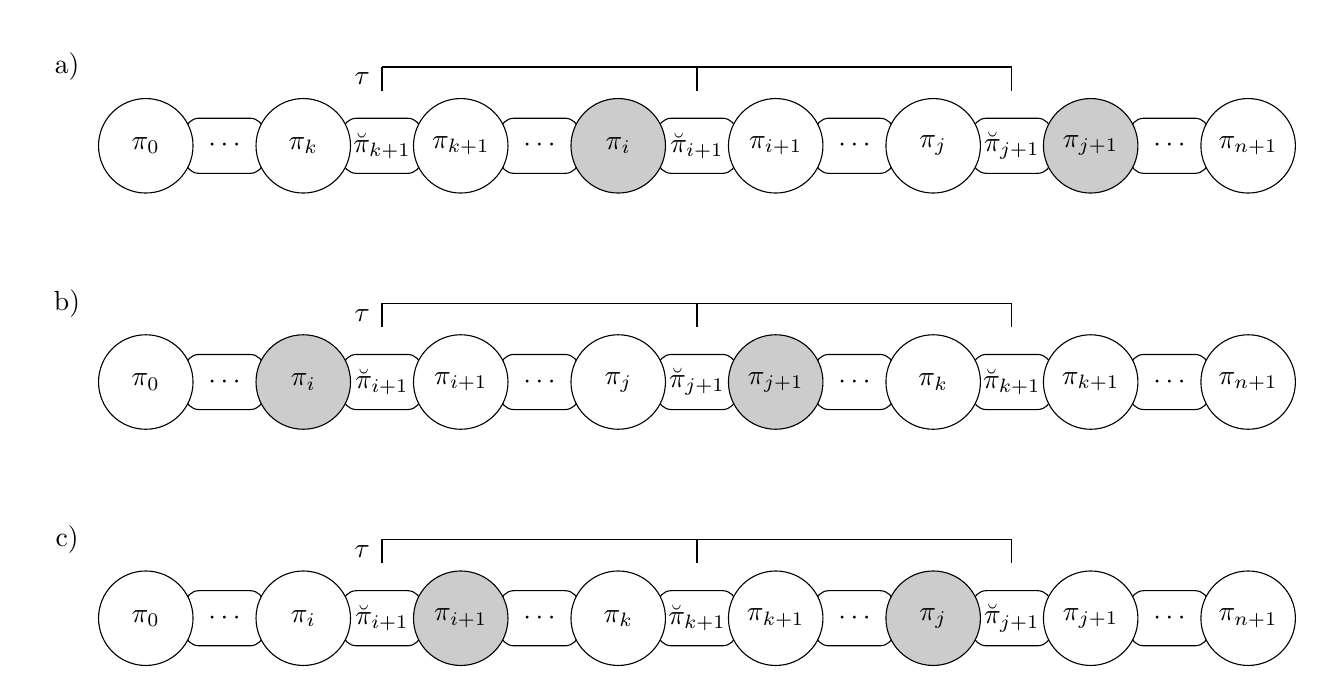
\begin{tikzpicture}
      %%%%% a)

      \node[draw=none,fill=none, minimum height=1cm, minimum width=1cm] at (-3.0, -2.0) {a)};

      % intergenic regions
      \node[rectangle,draw,fill=white!20, minimum height=.7cm, minimum width=1cm, rounded corners=5pt] at (-1.0, -3.0) {$\cdots$};
      \node[rectangle,draw,fill=white!20, minimum height=.7cm, minimum width=1cm, rounded corners=5pt] at (1.0, -3.0) {$\breve\pi_{k+1}$};
      \node[rectangle,draw,fill=white!20, minimum height=.7cm, minimum width=1cm, rounded corners=5pt] at (3.0, -3.0) {$\cdots$};
      \node[rectangle,draw,fill=white!20, minimum height=.7cm, minimum width=1cm, rounded corners=5pt] at (5.0, -3.0) {$\breve\pi_{i+1}$};
      \node[rectangle,draw,fill=white!20, minimum height=.7cm, minimum width=1cm, rounded corners=5pt] at (7.0, -3.0) {$\cdots$};
      \node[rectangle,draw,fill=white!20, minimum height=.7cm, minimum width=1cm, rounded corners=5pt] at (9.0, -3.0) {$\breve\pi_{j+1}$};
      \node[rectangle,draw,fill=white!20, minimum height=.7cm, minimum width=1cm, rounded corners=5pt] at (11.0, -3.0) {$\cdots$};

      % genes
      \node[draw, circle, minimum height=1.2cm, minimum width=1.2cm, fill=white!20] at ({(2*0 - 2)}, -3.0) {$\pi_{0}$};
      \node[draw, circle, minimum height=1.2cm, minimum width=1.2cm, fill=white!20] at ({(2*1 - 2)}, -3.0) {$\pi_{k}$};
      \node[draw, circle, minimum height=1.2cm, minimum width=1.2cm, fill=white!20] at ({(2*2 - 2)}, -3.0) {$\pi_{k+1}$};
      \node[draw, circle, minimum height=1.2cm, minimum width=1.2cm, fill=black!20] at ({(2*3 - 2)}, -3.0) {$\pi_{i}$};
      \node[draw, circle, minimum height=1.2cm, minimum width=1.2cm, fill=white!20] at ({(2*4 - 2)}, -3.0) {$\pi_{i+1}$};
      \node[draw, circle, minimum height=1.2cm, minimum width=1.2cm, fill=white!20] at ({(2*5 - 2)}, -3.0) {$\pi_{j}$};
      \node[draw, circle, minimum height=1.2cm, minimum width=1.2cm, fill=black!20] at ({(2*6 - 2)}, -3.0) {$\pi_{j+1}$};
      \node[draw, circle, minimum height=1.2cm, minimum width=1.2cm, fill=white!20] at ({(2*7 - 2)}, -3.0) {$\pi_{n+1}$};

      % indexes
      \draw (1.0, -2.3) -- (1.0, -2.0);
      \draw (5.0, -2.3) -- (5.0, -2.0);
      \draw (9.0, -2.3) -- (9.0, -2.0);
      \draw (1.0, -2.0) -- (9.0, -2.0);
      \node[draw=none,fill=none] at (0.75, -2.15) {$\tau$};

      %%%%% b)

      \node[draw=none,fill=none, minimum height=1cm, minimum width=1cm] at (-3.0, -5.0) {b)};

      % intergenic regions
      \node[rectangle,draw,fill=white!20, minimum height=.7cm, minimum width=1cm, rounded corners=5pt] at (-1.0, -6.0) {$\cdots$};
      \node[rectangle,draw,fill=white!20, minimum height=.7cm, minimum width=1cm, rounded corners=5pt] at (1.0, -6.0) {$\breve\pi_{i+1}$};
      \node[rectangle,draw,fill=white!20, minimum height=.7cm, minimum width=1cm, rounded corners=5pt] at (3.0, -6.0) {$\cdots$};
      \node[rectangle,draw,fill=white!20, minimum height=.7cm, minimum width=1cm, rounded corners=5pt] at (5.0, -6.0) {$\breve\pi_{j+1}$};
      \node[rectangle,draw,fill=white!20, minimum height=.7cm, minimum width=1cm, rounded corners=5pt] at (7.0, -6.0) {$\cdots$};
      \node[rectangle,draw,fill=white!20, minimum height=.7cm, minimum width=1cm, rounded corners=5pt] at (9.0, -6.0) {$\breve\pi_{k+1}$};
      \node[rectangle,draw,fill=white!20, minimum height=.7cm, minimum width=1cm, rounded corners=5pt] at (11.0, -6.0) {$\cdots$};

      % genes
      \node[draw, circle, minimum height=1.2cm, minimum width=1.2cm, fill=white!20] at ({(2*0 - 2)}, -6.0) {$\pi_{0}$};
      \node[draw, circle, minimum height=1.2cm, minimum width=1.2cm, fill=black!20] at ({(2*1 - 2)}, -6.0) {$\pi_{i}$};
      \node[draw, circle, minimum height=1.2cm, minimum width=1.2cm, fill=white!20] at ({(2*2 - 2)}, -6.0) {$\pi_{i+1}$};
      \node[draw, circle, minimum height=1.2cm, minimum width=1.2cm, fill=white!20] at ({(2*3 - 2)}, -6.0) {$\pi_{j}$};
      \node[draw, circle, minimum height=1.2cm, minimum width=1.2cm, fill=black!20] at ({(2*4 - 2)}, -6.0) {$\pi_{j+1}$};
      \node[draw, circle, minimum height=1.2cm, minimum width=1.2cm, fill=white!20] at ({(2*5 - 2)}, -6.0) {$\pi_{k}$};
      \node[draw, circle, minimum height=1.2cm, minimum width=1.2cm, fill=white!20] at ({(2*6 - 2)}, -6.0) {$\pi_{k+1}$};
      \node[draw, circle, minimum height=1.2cm, minimum width=1.2cm, fill=white!20] at ({(2*7 - 2)}, -6.0) {$\pi_{n+1}$};

      % indexes
      \draw (1.0, -5.3) -- (1.0, -5.0);
      \draw (5.0, -5.3) -- (5.0, -5.0);
      \draw (9.0, -5.3) -- (9.0, -5.0);
      \draw (1.0, -5.0) -- (9.0, -5.0);
      \node[draw=none,fill=none] at (0.75, -5.15) {$\tau$};

      %%%%% c)

      \node[draw=none,fill=none, minimum height=1cm, minimum width=1cm] at (-3.0, -8.0) {c)};

      % intergenic regions
      \node[rectangle,draw,fill=white!20, minimum height=.7cm, minimum width=1cm, rounded corners=5pt] at (-1.0, -9.0) {$\cdots$};
      \node[rectangle,draw,fill=white!20, minimum height=.7cm, minimum width=1cm, rounded corners=5pt] at (1.0, -9.0) {$\breve\pi_{i+1}$};
      \node[rectangle,draw,fill=white!20, minimum height=.7cm, minimum width=1cm, rounded corners=5pt] at (3.0, -9.0) {$\cdots$};
      \node[rectangle,draw,fill=white!20, minimum height=.7cm, minimum width=1cm, rounded corners=5pt] at (5.0, -9.0) {$\breve\pi_{k+1}$};
      \node[rectangle,draw,fill=white!20, minimum height=.7cm, minimum width=1cm, rounded corners=5pt] at (7.0, -9.0) {$\cdots$};
      \node[rectangle,draw,fill=white!20, minimum height=.7cm, minimum width=1cm, rounded corners=5pt] at (9.0, -9.0) {$\breve\pi_{j+1}$};
      \node[rectangle,draw,fill=white!20, minimum height=.7cm, minimum width=1cm, rounded corners=5pt] at (11.0, -9.0) {$\cdots$};

      % genes
      \node[draw, circle, minimum height=1.2cm, minimum width=1.2cm, fill=white!20] at ({(2*0 - 2)}, -9.0) {$\pi_{0}$};
      \node[draw, circle, minimum height=1.2cm, minimum width=1.2cm, fill=white!20] at ({(2*1 - 2)}, -9.0) {$\pi_{i}$};
      \node[draw, circle, minimum height=1.2cm, minimum width=1.2cm, fill=black!20] at ({(2*2 - 2)}, -9.0) {$\pi_{i+1}$};
      \node[draw, circle, minimum height=1.2cm, minimum width=1.2cm, fill=white!20] at ({(2*3 - 2)}, -9.0) {$\pi_{k}$};
      \node[draw, circle, minimum height=1.2cm, minimum width=1.2cm, fill=white!20] at ({(2*4 - 2)}, -9.0) {$\pi_{k+1}$};
      \node[draw, circle, minimum height=1.2cm, minimum width=1.2cm, fill=black!20] at ({(2*5 - 2)}, -9.0) {$\pi_{j}$};
      \node[draw, circle, minimum height=1.2cm, minimum width=1.2cm, fill=white!20] at ({(2*6 - 2)}, -9.0) {$\pi_{j+1}$};
      \node[draw, circle, minimum height=1.2cm, minimum width=1.2cm, fill=white!20] at ({(2*7 - 2)}, -9.0) {$\pi_{n+1}$};

      % indexes
      \draw (1.0, -8.3) -- (1.0, -8.0);
      \draw (5.0, -8.3) -- (5.0, -8.0);
      \draw (9.0, -8.3) -- (9.0, -8.0);
      \draw (1.0, -8.0) -- (9.0, -8.0);
      \node[draw=none,fill=none] at (0.75, -8.15) {$\tau$};
    \end{tikzpicture}
  }
  \caption[Exemplo de remoção de, pelo menos, um breakpoint tipo um após a aplicação de uma transposição $\tau$.]{Exemplo de remoção de, pelo menos, um breakpoint tipo um após a aplicação de uma transposição $\tau$.}
  \label{figure:WDJFPAXN}
\end{figure}

A seguir apresentamos o Algoritmo~\ref{algorithm:SAAUGXYG} para a variação sem sinais do problema \SbIRT{}.

\begin{algorithm}[!tbh]
  \caption{Um algoritmo de aproximação para o problema \SbIR{}.\label{algorithm:SAAUGXYG}}
  \Entrada{Uma instância intergênica rígida balanceada sem sinais $\mathcal{I}=((\pi,\breve\pi),(\iota,\breve\iota))$}
  \Saida{Uma sequência de reversões e transposições $S$, tal que $(\pi,\breve\pi) \cdot S = (\iota,\breve\iota)$}
    Seja $S \gets ()$ \\
    \Enqto{$ib(\mathcal{I}) > 1$}{
      \tcp{Lema~\ref{lemma:WYEZMYTM}}
      $(\pi_i,\pi_{i+1})$, $(\pi_j,\pi_{j+1}) \gets $ encontre um par de breakpoints conectados \\
      \tcp{Lema~\ref{lemma:SIAFJFDO}}
      \Se{$(\pi_i,\pi_{i+1})$, $(\pi_j,\pi_{j+1})$ pertence ao caso $i$}{
        $S' \gets (\rho_1)$ \\
      }\SenaoSe{$(\pi_i,\pi_{i+1})$, $(\pi_j,\pi_{j+1})$ pertence ao caso $ii$}{
        $S' \gets (\tau_1)$ \\
      }\SenaoSe{$(\pi_i,\pi_{i+1})$, $(\pi_j,\pi_{j+1})$ pertence ao caso $iii$}{
        $S' \gets (\tau_1)$ \\
      }\SenaoSe{$(\pi_i,\pi_{i+1})$, $(\pi_j,\pi_{j+1})$ pertence ao caso $iv$}{
        $S' \gets (\rho_1,\rho_2)$ \\
      }
      $S \gets S + S'$ \\
      $\mathcal{I} \gets ((\pi, \breve\pi) \cdot S',(\iota,\breve\iota))$ \\
    }
  \Retorna{S}
\end{algorithm}

\begin{lemma}\label{lemma:QMLCZMMK}
Dada uma instância intergênica rígida balanceada sem sinais $\mathcal{I}=((\pi,\breve\pi),\break(\iota,\breve\iota))$, o Algoritmo~\ref{algorithm:SAAUGXYG} transforma $(\pi,\breve\pi)$ em $(\iota,\breve\iota)$ utilizando no máximo $2ib_1(\mathcal{I})$ eventos de reversão e transposição.
\end{lemma}
\begin{proof}
  No Algoritmo~\ref{algorithm:SAAUGXYG}, temos que enquanto $ib_1(\mathcal{I})$ for maior que um, ou seja, $(\pi,\breve\pi)$ for diferente de $(\iota,\breve\iota)$ (pela Observação~\ref{remark:UDYJTHAH} e Lema~\ref{lemma:WSPRPLAH}), o seguinte procedimento é aplicado: pelos lemas~\ref{lemma:WYEZMYTM} e~\ref{lemma:SIAFJFDO}, sempre podemos encontrar um par conectado de breakpoints e remover pelo menos um breakpoint tipo um após aplicar no máximo duas reversões ou uma transposição. A cada iteração do algoritmo pelo menos um breakpoint tipo um é removido. Dessa forma, o genoma alvo eventualmente será alcançado. No pior caso, cada breakpoint tipo um é removido utilizando dois eventos de rearranjo. Logo, uma sequência com, no máximo, $2ib_1(\mathcal{I})$ reversões e transposições é utilizada para transformar $(\pi,\breve\pi)$ em $(\iota,\breve\iota)$ e o lema segue.
\end{proof}

Note que o Algoritmo~\ref{algorithm:SAAUGXYG} difere do Algoritmo~\ref{algorithm:AKKUXQNR} apenas pelos casos $ii$ e $iii$ de um par conectado de breakpoints, que também podem ser realizados em tempo linear. Logo, o tempo de execução do Algoritmo~\ref{algorithm:SAAUGXYG} também é $\mathcal{O}(n^2)$.

\begin{theorem}\label{theorem:ZEFRNBIE}
Dada uma instância intergênica rígida balanceada sem sinais $\mathcal{I}=\break((\pi,\breve\pi),(\iota,\breve\iota))$, o Algoritmo~\ref{algorithm:SAAUGXYG} é uma $6$-aproximação para o problema \SbIRT{}.
\end{theorem}
\begin{proof}
Pelo Lema~\ref{lemma:QMLCZMMK}, o Algoritmo~\ref{algorithm:SAAUGXYG} transforma $(\pi,\breve\pi)$ em $(\iota,\breve\iota)$ utilizando no máximo $2ib_1(\mathcal{I})$ eventos de reversão e transposição. Pelo Teorema~\ref{theorem:MPFPKHQO}, temos o seguinte limitante inferior $d_{\SbIRT}(\mathcal{I}) \ge \frac{ib_1(\mathcal{I})}{3}$. Logo, o teorema segue. 
\end{proof}

A seguir apresentaremos lemas que serão utilizados para obtermos algoritmos com melhores fatores de aproximação.

\begin{lemma}\label{lemma:RAJPFOWJ}
Dada uma representação intergênica rígida $(\pi,\breve\pi)$ e duas transposições consecutivas no formato:
$$(\pi,\breve\pi)\cdot\tau^{(i,j,k)}_{(\varphi_i,\varphi_j,\varphi_k)}\cdot\tau^{(i,i+k-j,k)}_{(\varphi^\prime_i,\varphi^\prime_{i+k-j},\varphi^\prime_k)},$$
então é possível realizar qualquer redistribuição de nucleotídeos nas regiões intergênicas $\breve\pi_i$, $\breve\pi_j$ e $\breve\pi_k$.
\end{lemma} 
\begin{proof}
Temos que mostrar que sempre é possível encontrar valores para as triplas $(\varphi_i,\varphi_j,\varphi_k)$ e $(\varphi^\prime_i,\varphi^\prime_{i+k-j},\varphi^\prime_k)$ para qualquer redistribuição de nucleotídeos nas regiões intergênicas $\breve\pi_i$, $\breve\pi_j$ e $\breve\pi_k$.

Como usamos apenas transposições, sabemos que $\breve\pi_i + \breve\pi_j + \breve\pi_k = \breve\pi^{\prime\prime}_i + \breve\pi^{\prime\prime}_j + \breve\pi^{\prime\prime}_k$, onde $\breve\pi^{\prime\prime}_i$, $\breve\pi^{\prime\prime}_j$ e $\breve \pi^{\prime\prime}_k$ representam os tamanhos das regiões intergênicas após a aplicação das duas transposições consecutivas.

Com base no fluxo de nucleotídeos entre as regiões intergênicas, realizaremos uma redução para uma instância $I_{MF}$ do problema de fluxo máximo, e mostraremos que sempre é possível encontrar uma solução para esta instância que satisfaça as restrições de redistribuição das regiões intergênicas $\breve\pi_i$, $\breve\pi_j$ e $\breve\pi_k$.

A Figura~\ref{figure:XUQWDNIW} (esquerda) mostra o fluxo que os nucleotídeos nas regiões intergênicas podem seguir ao aplicar as duas transposições consecutivas (declaradas no enunciado do Lemma~\ref{lemma:RAJPFOWJ}). Note que cada região intergênica pode enviar nucleotídeos para duas regiões intergênicas distintas. Assim, podemos criar um grafo, onde cada vértice corresponde a uma região intergênica, e onde existe um arco $(i,j)$ com capacidade ilimitada se a região intergênica $i$ pode enviar nucleotídeos para a região intergênica $j$.

Por fim, para obter a instância $I_{MF}$ do problema de fluxo máximo, adicionaremos os vértices 0 (origem) e 10 (destino), juntamente com os seguintes arcos: $(0,1)$, $(0, 2)$, $(0,3)$, $(7,10)$, $(8,10)$ e $(9,10)$ com suas respectivas capacidades: $a=\breve\pi_i$, $b=\breve\pi_j$, $c=\breve\pi_k$, $x=\breve\pi^{\prime\prime}_i$, $y=\breve\pi^{\prime\prime}_j $ e $z=\breve\pi^{\prime\prime}_k$. Todos os outros arcos têm capacidade infinita atribuída. Figura~\ref{figure:XUQWDNIW} (direita) mostra a instância $I_{MF}$ do problema de fluxo máximo obtido.

\begin{figure}[!tbh]
  \resizebox{.45\linewidth}{!}{
    \centering  
    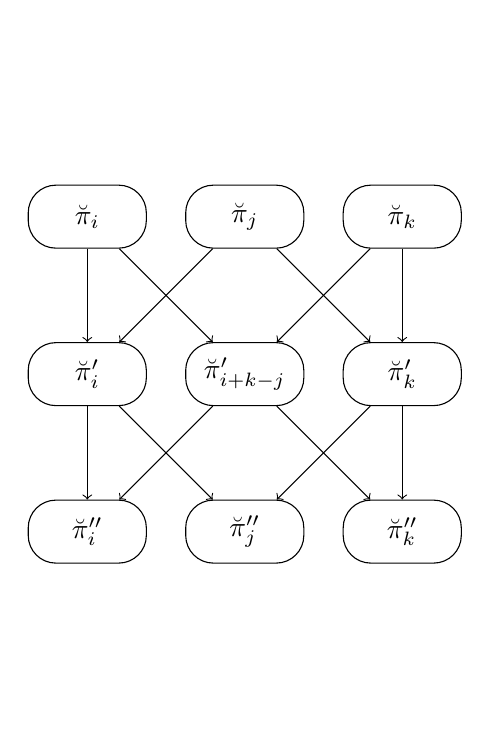
\begin{tikzpicture}
      \tikzstyle{STY1} = [draw, rectangle, minimum height=.8cm, minimum width=1.5cm, rounded corners=10pt]
      \tikzstyle{STY2} = [->]

      %%%%% VERTEX

      \node[draw=none, fill=none, rectangle, minimum height=.8cm, minimum width=1.5cm, rounded corners=10pt](v0) at ({(2*2 - 2)}, 2.0) {};

      \node[STY1](v1) at ({(2*1 - 2)}, 0.0) {$\breve\pi_i$};
      \node[STY1](v2) at ({(2*2 - 2)}, 0.0) {$\breve\pi_j$};
      \node[STY1](v3) at ({(2*3 - 2)}, 0.0) {$\breve\pi_k$};

      \node[STY1](v4) at ({(2*1 - 2)}, -2.0) {$\breve\pi^{\prime}_i$};
      \node[STY1](v5) at ({(2*2 - 2)}, -2.0) {$\breve\pi^{\prime}_{i+k-j}$};
      \node[STY1](v6) at ({(2*3 - 2)}, -2.0) {$\breve\pi^{\prime}_k$};


      \node[STY1](v7) at ({(2*1 - 2)}, -4.0) {$\breve\pi^{\prime\prime}_i$};
      \node[STY1](v8) at ({(2*2 - 2)}, -4.0) {$\breve\pi^{\prime\prime}_j$};
      \node[STY1](v9) at ({(2*3 - 2)}, -4.0) {$\breve\pi^{\prime\prime}_k$};

      \node[draw=none, fill=none, rectangle, minimum height=.8cm, minimum width=1.5cm, rounded corners=10pt](v10) at ({(2*2 - 2)}, -6.0) {};

      %%%%% EDGES

      \draw[STY2]  (v1) edge (v4);
      \draw[STY2]  (v1) edge (v5);
      \draw[STY2]  (v2) edge (v4);
      \draw[STY2]  (v2) edge (v6);
      \draw[STY2]  (v3) edge (v5);
      \draw[STY2]  (v3) edge (v6);

      \draw[STY2]  (v4) edge (v7);
      \draw[STY2]  (v4) edge (v8);
      \draw[STY2]  (v5) edge (v7);
      \draw[STY2]  (v5) edge (v9);
      \draw[STY2]  (v6) edge (v8);
      \draw[STY2]  (v6) edge (v9);
      %     \node[draw=none,fill=none, minimum height=1cm, minimum width=1cm] at (0.0, 2.0) {a)};
    \end{tikzpicture}
  }
  \hfill
  \resizebox{.45\linewidth}{!}{
    \centering
    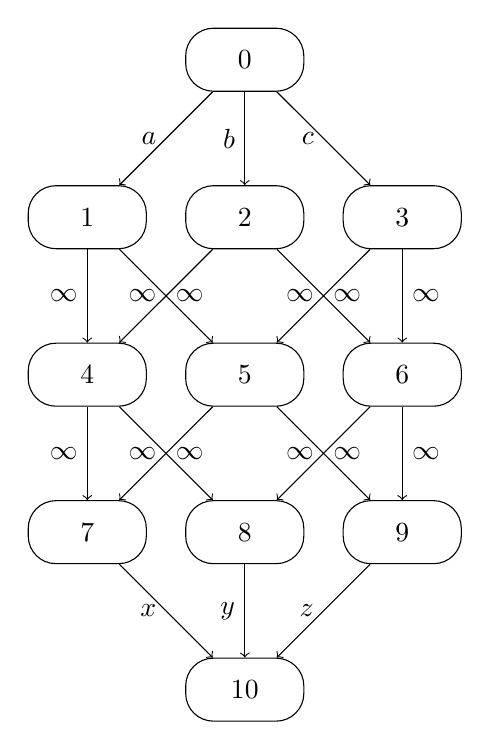
\begin{tikzpicture}
      \tikzstyle{STY1} = [draw, rectangle, minimum height=.8cm, minimum width=1.5cm, rounded corners=10pt]
      \tikzstyle{STY2} = [->]

      %%%%% VERTEX

      \node[STY1](v0) at ({(2*2 - 2)}, 2.0) {0};

      \node[STY1](v1) at ({(2*1 - 2)}, 0.0) {1};
      \node[STY1](v2) at ({(2*2 - 2)}, 0.0) {2};
      \node[STY1](v3) at ({(2*3 - 2)}, 0.0) {3};

      \node[STY1](v4) at ({(2*1 - 2)}, -2.0) {4};
      \node[STY1](v5) at ({(2*2 - 2)}, -2.0) {5};
      \node[STY1](v6) at ({(2*3 - 2)}, -2.0) {6};


      \node[STY1](v7) at ({(2*1 - 2)}, -4.0) {7};
      \node[STY1](v8) at ({(2*2 - 2)}, -4.0) {8};
      \node[STY1](v9) at ({(2*3 - 2)}, -4.0) {9};

      \node[STY1](v10) at ({(2*2 - 2)}, -6.0) {10};

      %%%%% EDGES
      \draw[STY2]  (v0) edge node[anchor=center, left, midway] {$a$} (v1);
      \draw[STY2]  (v0) edge node[anchor=center, left, midway] {$b$} (v2);
      \draw[STY2]  (v0) edge node[anchor=center, left, midway] {$c$} (v3);

      \draw[STY2]  (v1) edge node[anchor=center, left, midway] {$\infty$} (v4);
      \draw[STY2]  (v1) edge node[anchor=center, left, midway] {$\infty$} (v5);
      \draw[STY2]  (v2) edge node[anchor=center, right, midway] {$\infty$} (v4);
      \draw[STY2]  (v2) edge node[anchor=center, left, midway] {$\infty$} (v6);
      \draw[STY2]  (v3) edge node[anchor=center, right, midway] {$\infty$} (v5);
      \draw[STY2]  (v3) edge node[anchor=center, right, midway] {$\infty$} (v6);

      \draw[STY2]  (v4) edge node[anchor=center, left, midway] {$\infty$} (v7);
      \draw[STY2]  (v4) edge node[anchor=center, left, midway] {$\infty$} (v8);
      \draw[STY2]  (v5) edge node[anchor=center, right, midway] {$\infty$} (v7);
      \draw[STY2]  (v5) edge node[anchor=center, left, midway] {$\infty$} (v9);
      \draw[STY2]  (v6) edge node[anchor=center, right, midway] {$\infty$} (v8);
      \draw[STY2]  (v6) edge node[anchor=center, right, midway] {$\infty$} (v9);

      \draw[STY2]  (v7) edge node[anchor=center, left, midway] {$x$} (v10);
      \draw[STY2]  (v8) edge node[anchor=center, left, midway] {$y$} (v10);
      \draw[STY2]  (v9) edge node[anchor=center, left, midway] {$z$} (v10);

      %     \node[draw=none,fill=none, minimum height=1cm, minimum width=1cm] at (0.0, 2.0) {b)};
    \end{tikzpicture}
  }
  \caption[Exemplo de fluxo de nucleotídeos entre as regiões intergênicas.]{No lado esquerdo, uma representação do fluxo de nucleotídeos entre as regiões intergênicas. No lado direito, a instância $I_{MF}$ do problema de fluxo máximo com os vértices de origem (0) e destino (10).}
  \label{figure:XUQWDNIW}
\end{figure}

Se analisarmos a Figura~\ref{figure:XUQWDNIW} (direita), podemos ver que o fluxo máximo da instância $I_{MF}$ é limitado a $\max\{(a+b+c),(x+ y+z)\}$, mas sabemos que $(a+b+c) = (x+y+z) = F$. Observe também que se houver uma redistribuição das regiões intergênicas $\breve\pi_i$, $\breve\pi_j$ e $\breve\pi_k$ isso significa que a instância $I_{MF}$ tem uma solução onde o máximo fluxo é $F$. Por outro lado, podemos ver que se a instância $I_{MF}$ tiver uma solução com fluxo máximo de $F$ e todas as variáveis da solução forem inteiras, isso significa que é possível redistribuir as regiões intergênicas $\breve \pi_i$, $\breve\pi_j$ e $\breve\pi_k$.

Agora, mostraremos que a instância $I_{MF}$ sempre tem uma solução com fluxo máximo $F$, onde todas as variáveis da solução são inteiras. Vamos provar este resultado fornecendo uma solução para a instância $I_{MF}$, que é obtida em três etapas.

A etapa 1 consiste em remover os vértices 8 e 9 de $I_{MF}$ (Figura~\ref{figure:NCRGBSMG} (esquerda)), e resolver a instância usando Programação Linear (PL) para obter uma possível solução fracionária. Observe que o fluxo máximo para esta etapa é menor ou igual a $x$, pois $(a+b+c) \ge x$. Além disso, existe uma solução que atinge exatamente $x$ (por exemplo, envie $a$ pelo caminho $(1,4,7)$; envie $b$ pelo caminho $(2,4,7)$; envie $c$ pelo caminho $(3,5,7)$). Seja $X^{\prime}$ a matriz da solução, na qual $X^{\prime}_{i,j}$ representa o fluxo que vai do vértice $i$ ao vértice $j$ na solução. Sabemos que $(X^{\prime}_{0,1}+X^{\prime}_{0,2}+X^{\prime}_{0,3}) = x$ e $x \in \mathbb{N}$. Se $\{X^{\prime}_{0,1},X^{\prime}_{0,2},X^{\prime}_{0,3}\} \not\subset \mathbb {N}$, podemos obter valores inteiros para as variáveis $X^{\prime}_{0,1}$, $X^{\prime}_{0,2}$ e $X^{\prime }_{0,3}$ redistribuindo a parte fracionária entre os arcos, isso é possível porque sabemos que $(a+b+c) \ge x$. Como todos os caminhos que partem dos vértices 1, 2 e 3 e chegam ao vértice 7 têm capacidade ilimitada, podemos obter uma solução inteira para as variáveis restantes. Após este processo, obtemos uma solução inteira $X^{\prime}$ para a etapa 1.

A etapa 2 consiste em remover os vértices 7 e 9 de $I_{MF}$, e atualizar a capacidade dos arcos $(0,1)$, $(0,2)$ e $(0,3)$ para $a ^{\prime}=a-X^{\prime}_{0,1}$, $b^{\prime}=b-X^{\prime}_{0,2}$ e $c^{\prime} =c-X^{\prime}_{0,3}$, respectivamente (Figura~\ref{figure:NCRGBSMG} (centro)). Em outras palavras, levamos em consideração, para os arcos $(0,1)$, $(0,2)$ e $(0,3)$, as capacidades que já foram utilizadas na etapa 1. Observe que $a^{\prime}+b^{\prime}+c^{\prime} = a+b+c-x$, mas também sabemos que $a+b+c = x+y+z$, assim $a^{\prime}+b^{\prime}+c^{\prime} = a+b+c-x = y+z \geq y$. Observe que o fluxo máximo para esta etapa é menor ou igual a $y$, pois $a^{\prime}+b^{\prime}+c^{\prime} \ge y$, e existe uma solução que atinge exatamente $y$ (por exemplo, envie $a^{\prime}$ pelo caminho $(1,4,8)$; envie $b^{\prime}$ pelo caminho $(2,4,8) $; envie $c^{\prime}$ pelo caminho $(3,6,8)$). Similarmente ao processo realizado na etapa 1, resolvemos o problema para obter uma solução $X^{\prime\prime}$ onde o fluxo máximo é $y$ e todas as variáveis são inteiras.

A etapa 3 consiste em remover os vértices 7 e 8 de $I_{MF}$, e atualizar a capacidade dos arcos $(0,1)$, $(0,2)$ e $(0,3)$ para $a ^{\prime\prime}=a^{\prime}-X^{\prime\prime}_{0,1}$, $b^{\prime\prime}=b^{\prime}-X^ {\prime\prime}_{0,2}$ e $c^{\prime\prime}=c^{\prime}-X^{\prime\prime}_{0,3}$, respectivamente (Figura~\ref{figure:NCRGBSMG} (direita)). Em outras palavras, levamos em consideração, para os arcos $(0,1)$, $(0,2)$ e $(0,3)$, as capacidades que já foram utilizadas nas etapas~1 e~2. Observe que $a^{\prime\prime}+b^{\prime\prime}+c^{\prime\prime} = a+b+c-x-y$, mas também sabemos que $a+b+c = x +y+z$, portanto $a^{\prime\prime}+b^{\prime\prime}+c^{\prime\prime} = a+b+c-x-y = z$. Observe que o fluxo máximo para esta etapa é igual a $z$, pois $a^{\prime\prime}+b^{\prime\prime}+c^{\prime\prime} = z$, e existe uma solução que atinja exatamente $z$ (por exemplo, envie $a^{\prime\prime}$ pelo caminho $(1,5,9)$; envie $b^{\prime\prime}$ pelo caminho $ (2,6,9)$; envie $c^{\prime\prime}$ pelo caminho $(3,6,9)$). Da mesma forma que o processo realizado na etapa 1, resolvemos o problema para obter uma solução $X^{\prime\prime\prime}$ onde o fluxo máximo é $z$ e todas as variáveis são números inteiros.

\begin{figure}[!tbh]
  \resizebox{.3\linewidth}{!}{
    \centering
    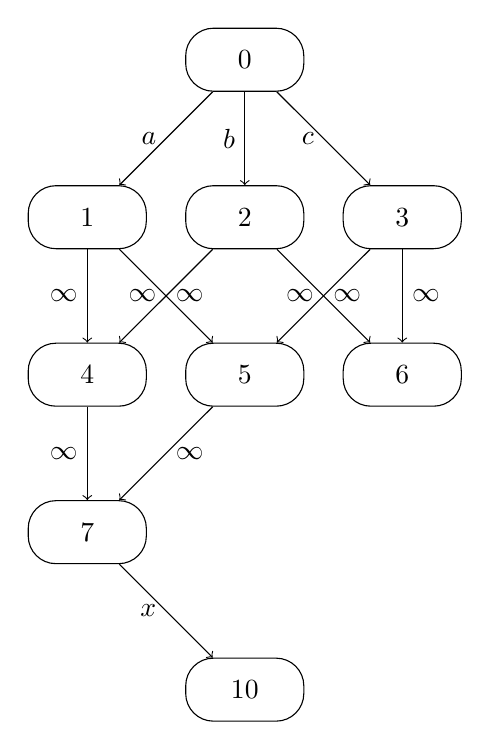
\begin{tikzpicture}
      \tikzstyle{STY1} = [draw, rectangle, minimum height=.8cm, minimum width=1.5cm, rounded corners=10pt]
      \tikzstyle{STY2} = [->]

      %%%%% VERTEX

      \node[STY1](v0) at ({(2*2 - 2)}, 2.0) {0};

      \node[STY1](v1) at ({(2*1 - 2)}, 0.0) {1};
      \node[STY1](v2) at ({(2*2 - 2)}, 0.0) {2};
      \node[STY1](v3) at ({(2*3 - 2)}, 0.0) {3};

      \node[STY1](v4) at ({(2*1 - 2)}, -2.0) {4};
      \node[STY1](v5) at ({(2*2 - 2)}, -2.0) {5};
      \node[STY1](v6) at ({(2*3 - 2)}, -2.0) {6};


      \node[STY1](v7) at ({(2*1 - 2)}, -4.0) {7};

      \node[STY1](v10) at ({(2*2 - 2)}, -6.0) {10};

      %%%%% EDGES
      \draw[STY2]  (v0) edge node[anchor=center, left, midway] {$a$} (v1);
      \draw[STY2]  (v0) edge node[anchor=center, left, midway] {$b$} (v2);
      \draw[STY2]  (v0) edge node[anchor=center, left, midway] {$c$} (v3);

      \draw[STY2]  (v1) edge node[anchor=center, left, midway] {$\infty$} (v4);
      \draw[STY2]  (v1) edge node[anchor=center, left, midway] {$\infty$} (v5);
      \draw[STY2]  (v2) edge node[anchor=center, right, midway] {$\infty$} (v4);
      \draw[STY2]  (v2) edge node[anchor=center, left, midway] {$\infty$} (v6);
      \draw[STY2]  (v3) edge node[anchor=center, right, midway] {$\infty$} (v5);
      \draw[STY2]  (v3) edge node[anchor=center, right, midway] {$\infty$} (v6);

      \draw[STY2]  (v4) edge node[anchor=center, left, midway] {$\infty$} (v7);
      \draw[STY2]  (v5) edge node[anchor=center, right, midway] {$\infty$} (v7);

      \draw[STY2]  (v7) edge node[anchor=center, left, midway] {$x$} (v10);

      %     \node[draw=none,fill=none, minimum height=1cm, minimum width=1cm] at (0.0, 2.0) {a)};
    \end{tikzpicture}
  }
  \hfill
  \resizebox{.3\linewidth}{!}{
    \centering
    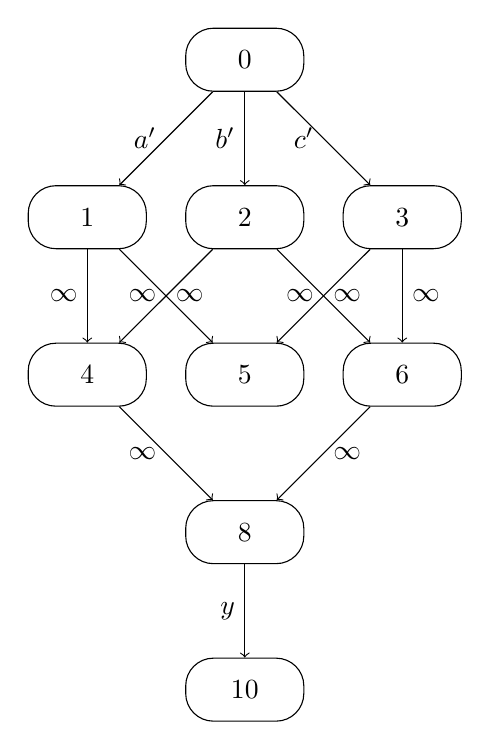
\begin{tikzpicture}
      \tikzstyle{STY1} = [draw, rectangle, minimum height=.8cm, minimum width=1.5cm, rounded corners=10pt]
      \tikzstyle{STY2} = [->]

      %%%%% VERTEX

      \node[STY1](v0) at ({(2*2 - 2)}, 2.0) {0};

      \node[STY1](v1) at ({(2*1 - 2)}, 0.0) {1};
      \node[STY1](v2) at ({(2*2 - 2)}, 0.0) {2};
      \node[STY1](v3) at ({(2*3 - 2)}, 0.0) {3};

      \node[STY1](v4) at ({(2*1 - 2)}, -2.0) {4};
      \node[STY1](v5) at ({(2*2 - 2)}, -2.0) {5};
      \node[STY1](v6) at ({(2*3 - 2)}, -2.0) {6};

      \node[STY1](v8) at ({(2*2 - 2)}, -4.0) {8};

      \node[STY1](v10) at ({(2*2 - 2)}, -6.0) {10};

      %%%%% EDGES
      \draw[STY2]  (v0) edge node[anchor=center, left, midway] {$a^{\prime}$} (v1);
      \draw[STY2]  (v0) edge node[anchor=center, left, midway] {$b^{\prime}$} (v2);
      \draw[STY2]  (v0) edge node[anchor=center, left, midway] {$c^{\prime}$} (v3);

      \draw[STY2]  (v1) edge node[anchor=center, left, midway] {$\infty$} (v4);
      \draw[STY2]  (v1) edge node[anchor=center, left, midway] {$\infty$} (v5);
      \draw[STY2]  (v2) edge node[anchor=center, right, midway] {$\infty$} (v4);
      \draw[STY2]  (v2) edge node[anchor=center, left, midway] {$\infty$} (v6);
      \draw[STY2]  (v3) edge node[anchor=center, right, midway] {$\infty$} (v5);
      \draw[STY2]  (v3) edge node[anchor=center, right, midway] {$\infty$} (v6);

      \draw[STY2]  (v4) edge node[anchor=center, left, midway] {$\infty$} (v8);
      \draw[STY2]  (v6) edge node[anchor=center, right, midway] {$\infty$} (v8);
      \draw[STY2]  (v8) edge node[anchor=center, left, midway] {$y$} (v10);

      %     \node[draw=none,fill=none, minimum height=1cm, minimum width=1cm] at (0.0, 2.0) {b)};
    \end{tikzpicture}
  }
  \hfill
  \resizebox{.3\linewidth}{!}{
    \centering
    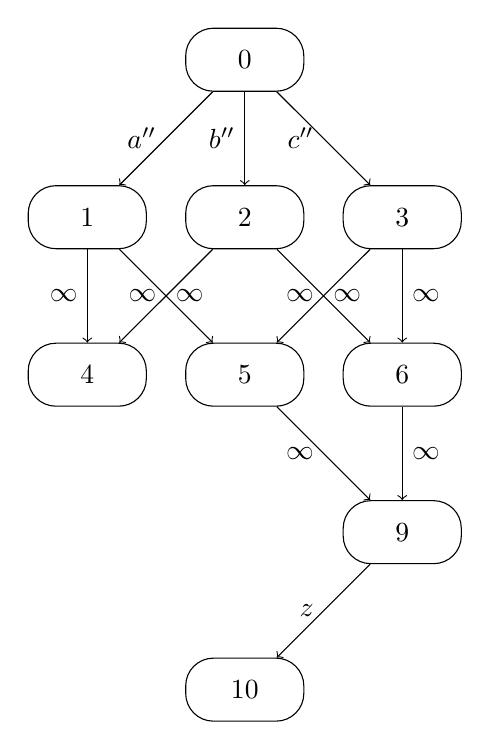
\begin{tikzpicture}
      \tikzstyle{STY1} = [draw, rectangle, minimum height=.8cm, minimum width=1.5cm, rounded corners=10pt]
      \tikzstyle{STY2} = [->]

      %%%%% VERTEX

      \node[STY1](v0) at ({(2*2 - 2)}, 2.0) {0};

      \node[STY1](v1) at ({(2*1 - 2)}, 0.0) {1};
      \node[STY1](v2) at ({(2*2 - 2)}, 0.0) {2};
      \node[STY1](v3) at ({(2*3 - 2)}, 0.0) {3};

      \node[STY1](v4) at ({(2*1 - 2)}, -2.0) {4};
      \node[STY1](v5) at ({(2*2 - 2)}, -2.0) {5};
      \node[STY1](v6) at ({(2*3 - 2)}, -2.0) {6};

      \node[STY1](v9) at ({(2*3 - 2)}, -4.0) {9};

      \node[STY1](v10) at ({(2*2 - 2)}, -6.0) {10};

      %%%%% EDGES
      \draw[STY2]  (v0) edge node[anchor=center, left, midway] {$a^{\prime\prime}$} (v1);
      \draw[STY2]  (v0) edge node[anchor=center, left, midway] {$b^{\prime\prime}$} (v2);
      \draw[STY2]  (v0) edge node[anchor=center, left, midway] {$c^{\prime\prime}$} (v3);

      \draw[STY2]  (v1) edge node[anchor=center, left, midway] {$\infty$} (v4);
      \draw[STY2]  (v1) edge node[anchor=center, left, midway] {$\infty$} (v5);
      \draw[STY2]  (v2) edge node[anchor=center, right, midway] {$\infty$} (v4);
      \draw[STY2]  (v2) edge node[anchor=center, left, midway] {$\infty$} (v6);
      \draw[STY2]  (v3) edge node[anchor=center, right, midway] {$\infty$} (v5);
      \draw[STY2]  (v3) edge node[anchor=center, right, midway] {$\infty$} (v6);

      \draw[STY2]  (v5) edge node[anchor=center, left, midway] {$\infty$} (v9);
      \draw[STY2]  (v6) edge node[anchor=center, right, midway] {$\infty$} (v9);
      \draw[STY2]  (v9) edge node[anchor=center, left, midway] {$z$} (v10);

      %     \node[draw=none,fill=none, minimum height=1cm, minimum width=1cm] at (0.0, 2.0) {c)};
    \end{tikzpicture}
  }
  \caption[Divisão da instância $I_{MF}$ do problema de fluxo máximo em três etapas.]{Divisão da instância $I_{MF}$ do problema de fluxo máximo em três etapas.}
  \label{figure:NCRGBSMG}
\end{figure}

A solução final $X$ consiste na soma de todas as capacidades utilizadas pelas soluções nas etapas 1, 2 e 3, ou seja, $\forall$~$1\leq i,j\leq 10$, $X_{i, j} = X^{\prime}_{i,j} + X^{\prime\prime}_{i,j} + X^{\prime\prime\prime}_{i,j}$. Observe que a solução $X$ não viola nenhuma restrição de capacidade, todas as variáveis são inteiras e o fluxo máximo é $F=a+b+c=x+y+z$.

\end{proof}

Em resumo, o Lema~\ref{lemma:RAJPFOWJ} nos permite, com duas transposições consecutivas, redistribuir o tamanho de três regiões intergênicas mantendo os genes na mesma ordem e orientação.

\begin{lemma}\label{lemma:FSGHLWJU}
Dada uma instância intergênica rígida balanceada sem sinais $\mathcal{I}=((\pi,\breve\pi),\break(\iota,\breve\iota))$ com pelo menos dois breakpoints sobrecarregados, então existe uma sequência de duas transposições que remove pelo menos dois breakpoints tipo um de $\mathcal{I}$.
\end{lemma}
\begin{proof}
Seja $(\pi_i,\pi_{i+1})$ e $(\pi_j,\pi_{j+1})$ dois breakpoints sobrecarregados de $\mathcal{I}$.
Agora, observe que deve existir um terceiro breakpoint tipo um $(\pi_k,\pi_{k+1})$ em $\mathcal{I}$. Caso contrário, $\mathcal{I}$ seria uma instância desbalanceada. Pelo Lema~\ref{lemma:RAJPFOWJ}, sabemos que é possível realizar qualquer redistribuição de nucleotídeos em três regiões intergênicas utilizando duas transposições consecutivas. Dessa forma, podemos realizar a redistribuição do tamanho das regiões intergênicas $\breve\pi_{i+1}$, $\breve\pi_{j+1}$ e $\breve\pi_{k+1}$ para $\breve\iota_{\max(\pi_i,\pi_{i+1})}$, $\breve\iota_{\max(\pi_j,\pi_{j+1})}$ e $\breve\pi_{k+1} + (\breve\pi_{i+1} - \breve\iota_{\max(\pi_i,\pi_{i+1})}) + (\breve\pi_{j+1} - \breve\iota_{\max(\pi_j,\pi_{j+1})})$, respectivamente. Neste caso, o excesso de nucleotídeos nos breakpoits sobrecarregados é transferido para o breakpoint $(\pi_k,\pi_{k+1})$. Como resultado, pelo menos dois breakpoints tipo um são removidos após a aplicação de duas transposições, e o lema segue.
\end{proof}

\begin{lemma}\label{lemma:RHTVEKOL}
Dada uma instância intergênica rígida balanceada sem sinais $\mathcal{I}=((\pi,\breve\pi),\break(\iota,\breve\iota))$ com pelo menos um breakpoint sobrecarregado $(\pi_i,\pi_{i+1})$ e pelo menos um breakpoint subcarregado $(\pi_j,\pi_{j+1})$, tal que $\breve\pi_{i+1} + \breve\pi_{j+1} \ge \breve\iota_{\max(\pi_i,\pi_{i+1})} + \breve\iota_{\max(\pi_j,\pi_{j+1})}$, então existe uma sequência de duas transposições que remove pelo menos dois breakpoints tipo um de $\mathcal{I}$.
\end{lemma}
\begin{proof}
Note que o excesso de nucleotídeos na região intergênica $\breve\pi_{i+1}$ é maior ou igual a quantidade de nucleotídeos que falta na região intergênica $\breve\pi_{j+1}$. Caso exista um terceiro breakpoint tipo um $(\pi_k,\pi_{k+1})$ em $\mathcal{I}$, então aplicamos o mesmo processo descrito no Lema~\ref{lemma:FSGHLWJU}. Caso contrário, selecionamos uma região intergênica $\breve\pi_{k+1}$ de forma que $k+1 \notin \{i+1,j+1\}$ e, pelo Lema~\ref{lemma:RAJPFOWJ}, realizamos a redistribuição do tamanho das regiões intergênicas $\breve\pi_{i+1}$, $\breve\pi_{j+1}$ e $\breve\pi_{k+1}$ para $\breve\iota_{\max(\pi_i,\pi_{i+1})}$, $\breve\iota_{\max(\pi_j,\pi_{j+1})}$ e $\breve\pi_{k+1}$, respectivamente. Note que a região intergênica $\breve\pi_{k+1}$ é utilizada apenas para transferir o excesso de nucleotídeos de $\breve\pi_{i+1}$ para $\breve\pi_{j+1}$, mas após a aplicação das duas transposições consecutivas seu tamanho permanece o mesmo. Como resultado, pelo menos dois breakpoints tipo um são removidos após a aplicação de duas transposições, e o lema segue.
\end{proof}

\begin{lemma}\label{lemma:ICDGSTEE}
Dada uma instância intergênica rígida balanceada sem sinais $\mathcal{I}=((\pi,\breve\pi),\break(\iota,\breve\iota))$ com apenas um breakpoint sobrecarregado $(\pi_i,\pi_{i+1})$ e sem breakpoints subcarregados $(\pi_j,\pi_{j+1})$, tal que $\breve\pi_{i+1} + \breve\pi_{j+1} \ge \breve\iota_{\max(\pi_i,\pi_{i+1})} + \breve\iota_{\max(\pi_j,\pi_{j+1})}$, então existe uma sequência de duas reversões que remove o breakpoint sobrecarregado $(\pi_i,\pi_{i+1})$ de $\mathcal{I}$ e não gera nenhum outro.
\end{lemma}
\begin{proof}
Note que um breakpoint sobrecarregado sempre vai estar conectado com qualquer outro breakpoint tipo um. Além disso, um segundo breakpoint tipo um $(\pi_k,\pi_{k+1})$ deve existir (subcarregado ou suave). Dessa forma, pelo caso $iv$ do Lema~\ref{lemma:IMYFBWDY}, temos que os breakpoints $(\pi_i,\pi_{i+1})$ e $(\pi_k,\pi_{k+1})$ estão conectados e o breakpoint sobrecarregado $(\pi_i,\pi_{i+1})$ é removido por uma sequência de duas reversões. Como não existe nenhum breakpoint subcarregado $(\pi_j,\pi_{j+1})$ em $\mathcal{I}$, tal que $\breve\pi_{i+1} + \breve\pi_{j+1} \ge \breve\iota_{\max(\pi_i,\pi_{i+1})} + \breve\iota_{\max(\pi_j,\pi_{j+1})}$, isso implica que a aplicação das duas reversões não gera breakpoints sobrecarregados, e o lema segue.
\end{proof}

\begin{lemma}\label{lemma:GZNXMCLB}
Dada uma instância intergênica rígida balanceada sem sinais $\mathcal{I}=((\pi,\breve\pi),\break(\iota,\breve\iota))$ sem breakpoints sobrecarregados e com $ib_1(\mathcal{I}) > 0$, então deve existir em $\mathcal{I}$ pelo menos um par suavemente conectado de breakpoints.
\end{lemma}
\begin{proof}
Suponha por contradição que $\mathcal{I}=((\pi,\breve\pi),(\iota,\breve\iota))$ sem breakpoints sobrecarregados e $ib_1(\mathcal{I}) > 0$ é uma instância intergênica rígida balanceada sem sinais, sem breakpoints sobrecarregados, com $ib_1(\mathcal{I}) > 0$ e não existe em  $\mathcal{I}$ um par suavemente conectado de breakpoints. Como $\mathcal{I}$ não possui breakpoints sobrecarregados, devem existir pelo menos dois breakpoints suaves. Caso contrário, $\mathcal{I}$ teria apenas breakpoints subcarregados e isso implicaria que $\mathcal{I}$ é uma instância desbalanceada, ou seja, $\sum_{i=1}^{n+1}\breve\pi_i < \sum_{i=1}^{n+1}\breve\iota_i$, o que contradiz a suposição de que $\mathcal{I}$ é uma instância intergênica rígida balanceada. Entretanto, como não existe em  $\mathcal{I}$ um par suavemente conectado de breakpoints, isso significa que os nucleotídeos presentes nas regiões intergênicas dos breakpoints suaves não é suficiente para removê-los sem torná-los em breakpoints subcarregados. Logo, temos que $\sum_{i=1}^{n+1}\breve\pi_i < \sum_{i=1}^{n+1}\breve\iota_i$, o que contradiz a suposição de que $\mathcal{I}$ é uma instância intergênica rígida balanceada.
\end{proof}

\begin{lemma}\label{lemma:LRCEAVRZ}
Dada uma instância intergênica rígida sem sinais $\mathcal{I}=((\pi,\breve\pi),(\iota,\breve\iota))$ e sejam $(\pi_i,\pi_{i+1})$ e $(\pi_j,\pi_{j+1})$ breakpoints suavemente conectados, então é possível remover pelo menos um breakpoint tipo um de $\mathcal{I}$ utilizando no máximo uma reversão ou uma transposição.
\end{lemma}
\begin{proof}
O Lema~\ref{lemma:SIAFJFDO} apresenta os quatro casos que abrangem todas as possibilidades a partir de um par conectado de breakpoints. Em particular, os casos $i$, $ii$ e $iii$ são os únicos em que é possível que ambos os breakpoints tipo um sejam suaves. Nos três casos apenas uma reversão ou uma transposição é utilizada para remover pelo menos um breakpoint tipo um de $\mathcal{I}$. Logo, o lema segue.
\end{proof}

A seguir apresentamos o Algoritmo~\ref{algorithm:JQHVZACM} para a variação sem sinais do problema \SbIRT{}.

\begin{algorithm}[!tbh]
  \caption{Um algoritmo de aproximação para o problema \SbIRT{}.\label{algorithm:JQHVZACM}}
  \Entrada{Uma instância intergênica rígida balanceada sem sinais $\mathcal{I}=((\pi,\breve\pi),(\iota,\breve\iota))$}
  \Saida{Uma sequência de reversões e transposições $S$, tal que $(\pi,\breve\pi) \cdot S = (\iota,\breve\iota)$}
    Seja $S \gets ()$ \\
    \Enqto{$ib_1(\mathcal{I}) > 1$}{
      \Se{existir pelo menos dois breakpoints sobrecarregados em $\mathcal{I}$}{
        \tcp{Lema~\ref{lemma:FSGHLWJU}}
        $S' \gets (\tau_1,\tau_2)$ \\
      }
      \SenaoSe{existir apenas um breakpoint sobrecarregado $(\pi_i,\pi_{i+1})$ em $\mathcal{I}$}{
        \Se{existir um breakpoint subcarregado $(\pi_j,\pi_{j+1})$ em $\mathcal{I}$, tal que $\breve\pi_{i+1} + \breve\pi_{j+1} \ge \breve\iota_{x} + \breve\iota_{y}$, onde $x = \max(\pi_i,\pi_{i+1})$ e $y=\max(\pi_j,\pi_{j+1})$}{
          \tcp{Lema~\ref{lemma:RHTVEKOL}}
          $S' \gets (\tau_1,\tau_2)$ ou $(\rho_1,\rho_2)$ \\
        }\Senao{
          \tcp{Lema~\ref{lemma:ICDGSTEE}}
          $S' \gets (\rho_1,\rho_2)$ \\
        }
      }\Senao{
        \tcp{Lemas~\ref{lemma:GZNXMCLB} e~\ref{lemma:LRCEAVRZ}}
        $(\pi_i,\pi_{i+1})$, $(\pi_j,\pi_{j+1}) \gets $ encontre um par suavemente conectado de breakpoints \\
        \Se{$(\pi_i,\pi_{i+1})$, $(\pi_j,\pi_{j+1})$ pertence ao caso $(i)$}{
          $S' \gets (\rho_1)$ \\
        }\SenaoSe{$(\pi_i,\pi_{i+1})$, $(\pi_j,\pi_{j+1})$ pertence ao caso $(ii)$}{
          $S' \gets (\tau_1)$ \\
        }\SenaoSe{$(\pi_i,\pi_{i+1})$, $(\pi_j,\pi_{j+1})$ pertence ao caso $(iii)$}{
          $S' \gets (\tau_1)$ \\
        }
      }
      $S \gets S + S'$ \\
      $\mathcal{I} \gets ((\pi, \breve\pi) \cdot S',(\iota,\breve\iota))$ \\

    }
  \Retorna{S}
\end{algorithm}

\begin{lemma}\label{lemma:RNJHXOWZ}
Dada uma instância intergênica rígida balanceada sem sinais $\mathcal{I}=((\pi,\breve\pi),\break(\iota,\breve\iota))$, o Algoritmo~\ref{algorithm:JQHVZACM} transforma $(\pi,\breve\pi)$ em $(\iota,\breve\iota)$ utilizando no máximo $\frac{3ib_1(\mathcal{I})}{2}$ eventos de reversão e transposição.
\end{lemma}
\begin{proof}
Podemos realizar a análise de cada iteração do Algoritmo~\ref{algorithm:JQHVZACM} considerando duas fases:
\begin{itemize}
  \item A remoção de breakpoints sobrecarregados: Caso existam dois ou mais breakpoints sobrecarregados em $\mathcal{I}$ duas transposições são aplicadas removendo dois breakpoints sobrecarregados (linhas 3-4). Caso exista apenas um breakpoint sobrecarregado em $\mathcal{I}$, então é verificado se existe um breakpoint subcarregado de forma que o excesso de nucleotídeos na região intergênica do breakpoint sobrecarregado seja suficiente para remover o breakpoint subcarregado. Caso exista, duas transposições são aplicadas removendo o tanto o breakpoint sobrecarregado como o subcarregado (linhas 6-7). Caso contrário, o breakpoint sobrecarregado é removido com duas reversões sem gerar nenhum breakpoint sobrecarregado (linhas 8-9).
  \item A remoção de breakpoints suaves: Se algoritmo chegou até esse ponto isso significa que não existe nenhum breakpoint sobrecarregado em $\mathcal{I}$ e deve existir pelo menos um par suavemente conectado de breakpoints. Dado um par suavemente conectado de breakpoints, então é possível remover um breakpoint tipo um utilizando no máximo uma reversão ou uma transposição.
\end{itemize}
Note que, a cada iteração do Algoritmo~\ref{algorithm:JQHVZACM}, pelo menos um breakpoint tipo um é removido. Dessa forma, o genoma alvo eventualmente será alcançado. Além disso, observe que, no pior caso, pelo menos um breakpoint tipo um é removido por duas reversões na fase de remoção de breakpoints sobrecarregados e pelo menos um breakpoint tipo um é removido por uma reversão ou uma transposição na fase de remoção de breakpoints suaves. Entretanto, se o pior caso da fase de remoção de breakpoints sobrecarregados ocorrer, sabemos que: i) o genoma alvo ainda não foi alcançado, ou seja, $(\pi,\breve\pi)$ é diferente de $(\iota,\breve\iota)$; ii) $\mathcal{I}$ não possui mais nenhum breakpoint sobrecarregado. Com essas duas constatações temos que o pior caso da fase de remoção de breakpoints sobrecarregados é obrigatoriamente seguido por uma fase de remoção de breakpoints suaves. Logo, no pior caso, temos que pelo menos dois breakpoints tipo um são removidos após a aplicação de no máximo três eventos de reverão e transposição. Como inicialmente $\mathcal{I}$ possui $ib_1(\mathcal{I})$ breakpoints tipo um, então no máximo $\frac{3ib_1(\mathcal{I})}{2}$ eventos de reversão e transposição são utilizados pelo Algoritmo~\ref{algorithm:JQHVZACM} para transformar $(\pi,\breve\pi)$ em $(\iota,\breve\iota)$, e o lema segue.
\end{proof}

Note que as fases de remoção de breakpoints sobrecarregados e suaves podem ser realizadas em tempo linear. Como a quantidade máxima de breakpoints tipo um em uma instância é $n+1$ e algoritmo, a cada iteração, remove pelo menos um breakpoint tipo um, então o tempo de execução do Algoritmo~\ref{algorithm:JQHVZACM} é $\mathcal{O}(n^2)$.


\begin{theorem}\label{theorem:QKJNIMOI}
Dada uma instância intergênica rígida balanceada sem sinais $\mathcal{I}=\break((\pi,\breve\pi),(\iota,\breve\iota))$, o Algoritmo~\ref{algorithm:JQHVZACM} é uma $4.5$-aproximação para o problema \SbIRT{}.
\end{theorem}
\begin{proof}
Pelo Lema~\ref{lemma:RNJHXOWZ}, o Algoritmo~\ref{algorithm:JQHVZACM} transforma $(\pi,\breve\pi)$ em $(\iota,\breve\iota)$ utilizando no máximo $\frac{3ib_1(\mathcal{I})}{2}$ eventos de reversão e transposição. Pelo Teorema~\ref{theorem:MPFPKHQO}, temos o seguinte limitante inferior $d_{\SbIRT}(\mathcal{I}) \ge \frac{ib_1(\mathcal{I})}{3}$. Logo, o teorema segue. 
\end{proof}